\documentclass[1p]{elsarticle_modified}
%\bibliographystyle{elsarticle-num}

%\usepackage[colorlinks]{hyperref}
%\usepackage{abbrmath_seonhwa} %\Abb, \Ascr, \Acal ,\Abf, \Afrak
\usepackage{amsfonts}
\usepackage{amssymb}
\usepackage{amsmath}
\usepackage{amsthm}
\usepackage{scalefnt}
\usepackage{amsbsy}
\usepackage{kotex}
\usepackage{caption}
\usepackage{subfig}
\usepackage{color}
\usepackage{graphicx}
\usepackage{xcolor} %% white, black, red, green, blue, cyan, magenta, yellow
\usepackage{float}
\usepackage{setspace}
\usepackage{hyperref}

\usepackage{tikz}
\usetikzlibrary{arrows}

\usepackage{multirow}
\usepackage{array} % fixed length table
\usepackage{hhline}

%%%%%%%%%%%%%%%%%%%%%
\makeatletter
\renewcommand*\env@matrix[1][\arraystretch]{%
	\edef\arraystretch{#1}%
	\hskip -\arraycolsep
	\let\@ifnextchar\new@ifnextchar
	\array{*\c@MaxMatrixCols c}}
\makeatother %https://tex.stackexchange.com/questions/14071/how-can-i-increase-the-line-spacing-in-a-matrix
%%%%%%%%%%%%%%%

\usepackage[normalem]{ulem}

\newcommand{\msout}[1]{\ifmmode\text{\sout{\ensuremath{#1}}}\else\sout{#1}\fi}
%SOURCE: \msout is \stkout macro in https://tex.stackexchange.com/questions/20609/strikeout-in-math-mode

\newcommand{\cancel}[1]{
	\ifmmode
	{\color{red}\msout{#1}}
	\else
	{\color{red}\sout{#1}}
	\fi
}

\newcommand{\add}[1]{
	{\color{blue}\uwave{#1}}
}

\newcommand{\replace}[2]{
	\ifmmode
	{\color{red}\msout{#1}}{\color{blue}\uwave{#2}}
	\else
	{\color{red}\sout{#1}}{\color{blue}\uwave{#2}}
	\fi
}

\newcommand{\Sol}{\mathcal{S}} %segment
\newcommand{\D}{D} %diagram
\newcommand{\A}{\mathcal{A}} %arc


%%%%%%%%%%%%%%%%%%%%%%%%%%%%%5 test

\def\sl{\operatorname{\textup{SL}}(2,\Cbb)}
\def\psl{\operatorname{\textup{PSL}}(2,\Cbb)}
\def\quan{\mkern 1mu \triangleright \mkern 1mu}

\theoremstyle{definition}
\newtheorem{thm}{Theorem}[section]
\newtheorem{prop}[thm]{Proposition}
\newtheorem{lem}[thm]{Lemma}
\newtheorem{ques}[thm]{Question}
\newtheorem{cor}[thm]{Corollary}
\newtheorem{defn}[thm]{Definition}
\newtheorem{exam}[thm]{Example}
\newtheorem{rmk}[thm]{Remark}
\newtheorem{alg}[thm]{Algorithm}

\newcommand{\I}{\sqrt{-1}}
\begin{document}

%\begin{frontmatter}
%
%\title{Boundary parabolic representations of knots up to 8 crossings}
%
%%% Group authors per affiliation:
%\author{Yunhi Cho} 
%\address{Department of Mathematics, University of Seoul, Seoul, Korea}
%\ead{yhcho@uos.ac.kr}
%
%
%\author{Seonhwa Kim} %\fnref{s_kim}}
%\address{Center for Geometry and Physics, Institute for Basic Science, Pohang, 37673, Korea}
%\ead{ryeona17@ibs.re.kr}
%
%\author{Hyuk Kim}
%\address{Department of Mathematical Sciences, Seoul National University, Seoul 08826, Korea}
%\ead{hyukkim@snu.ac.kr}
%
%\author{Seokbeom Yoon}
%\address{Department of Mathematical Sciences, Seoul National University, Seoul, 08826,  Korea}
%\ead{sbyoon15@snu.ac.kr}
%
%\begin{abstract}
%We find all boundary parabolic representation of knots up to 8 crossings.
%
%\end{abstract}
%\begin{keyword}
%    \MSC[2010] 57M25 
%\end{keyword}
%
%\end{frontmatter}

%\linenumbers
%\tableofcontents
%
\newcommand\colored[1]{\textcolor{white}{\rule[-0.35ex]{0.8em}{1.4ex}}\kern-0.8em\color{red} #1}%
%\newcommand\colored[1]{\textcolor{white}{ #1}\kern-2.17ex	\textcolor{white}{ #1}\kern-1.81ex	\textcolor{white}{ #1}\kern-2.15ex\color{red}#1	}

{\Large $\underline{12a_{0868}~(K12a_{0868})}$}

\setlength{\tabcolsep}{10pt}
\renewcommand{\arraystretch}{1.6}
\vspace{1cm}\begin{tabular}{m{100pt}>{\centering\arraybackslash}m{274pt}}
\multirow{5}{120pt}{
	\centering
	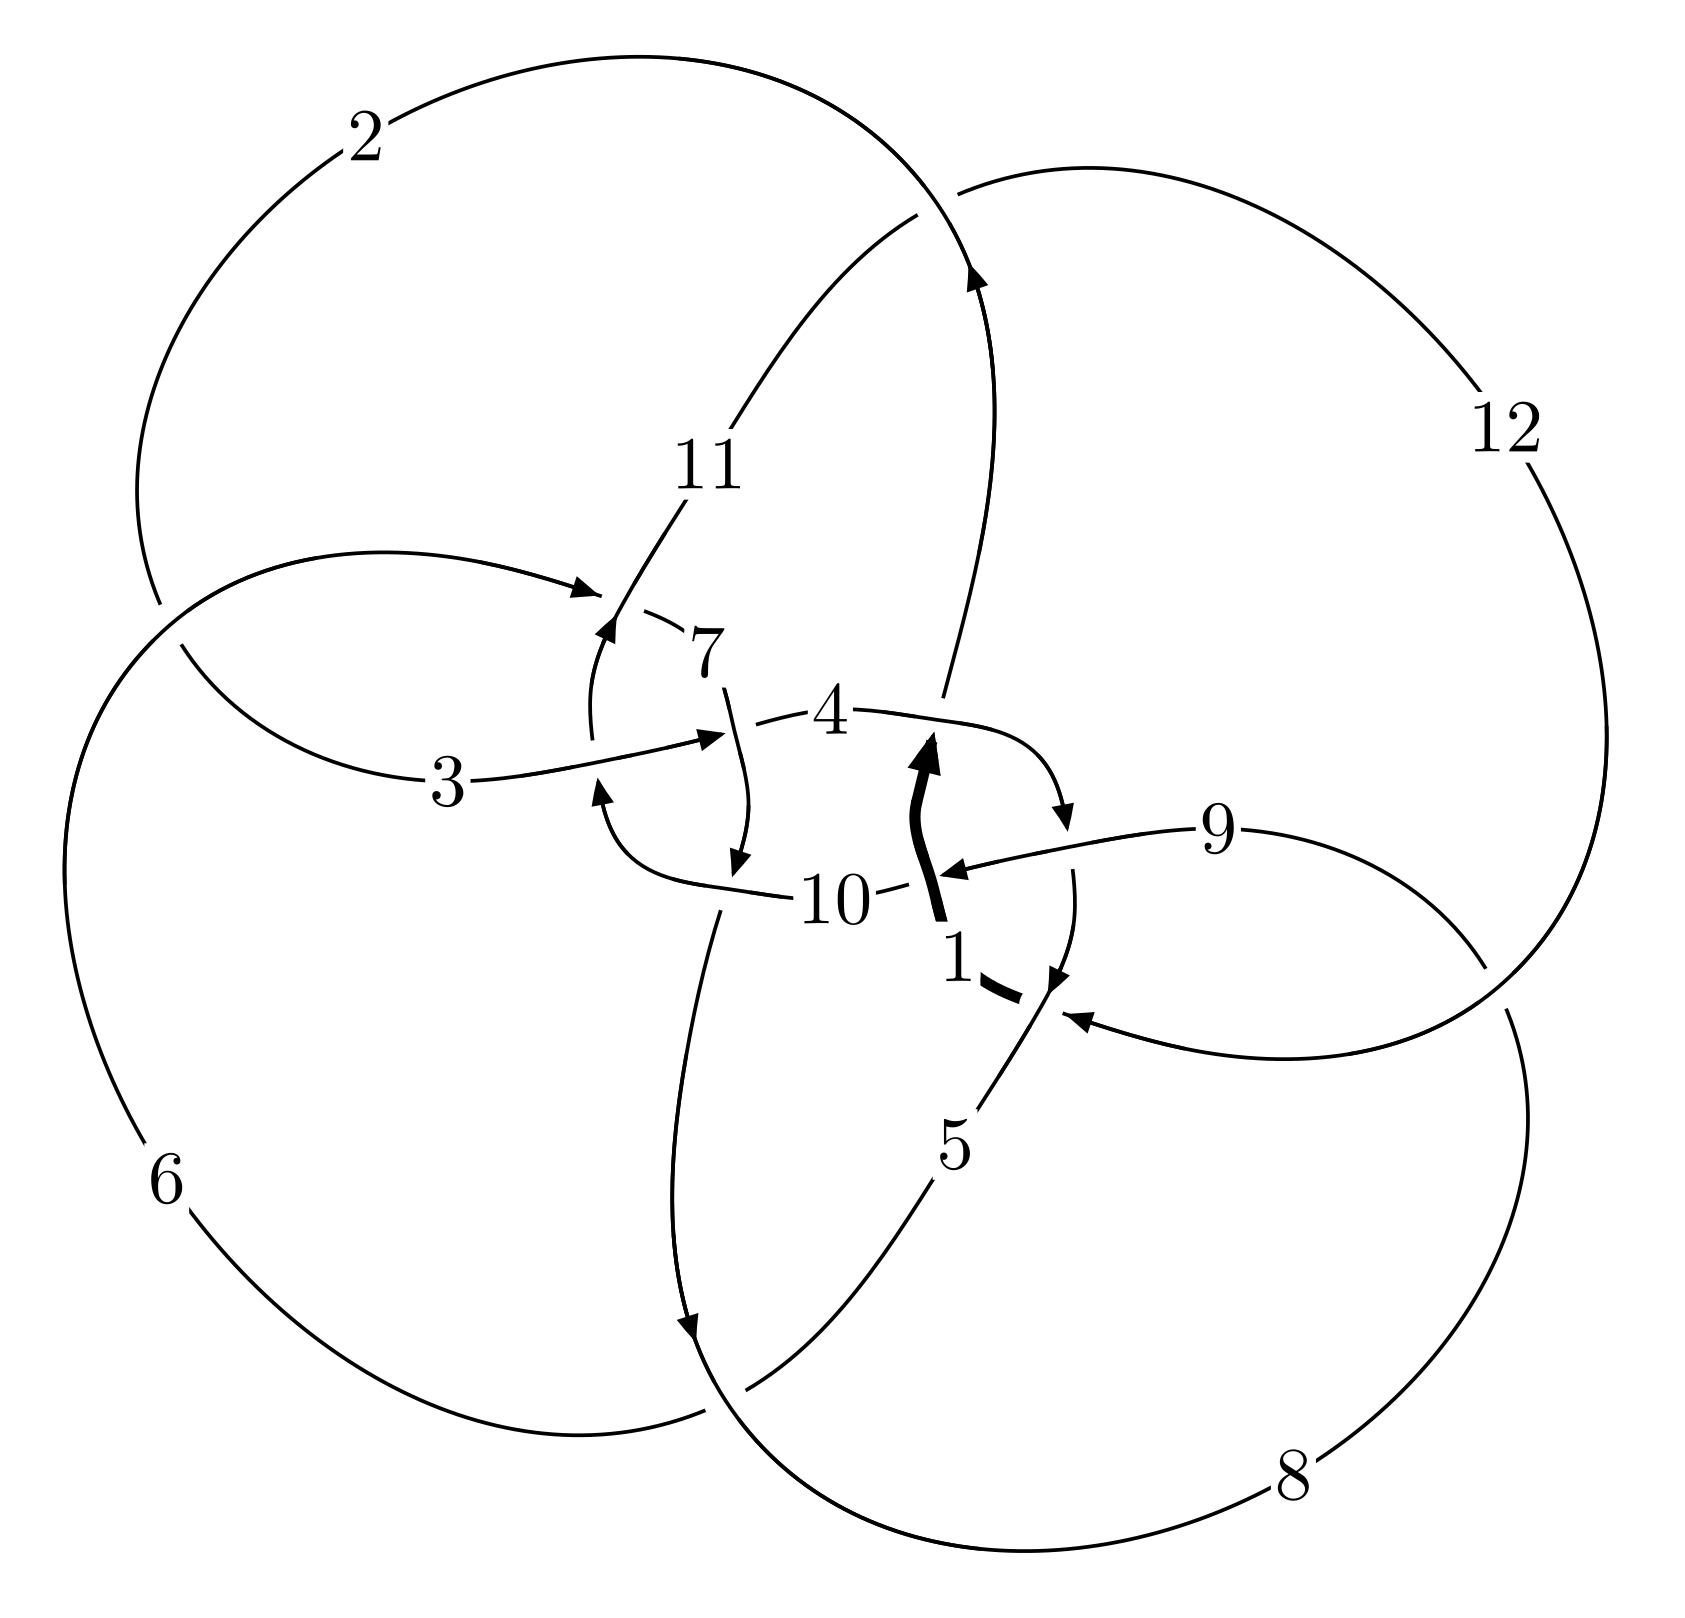
\includegraphics[width=112pt]{../../../GIT/diagram.site/Diagrams/png/1669_12a_0868.png}\\
\ \ \ A knot diagram\footnotemark}&
\allowdisplaybreaks
\textbf{Linearized knot diagam} \\
\cline{2-2}
 &
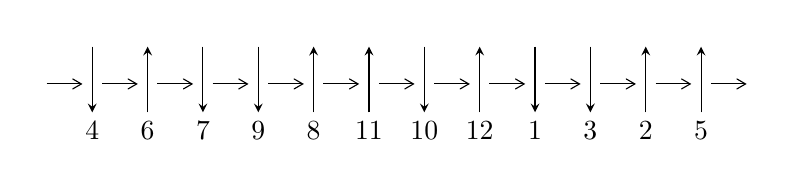
\begin{tikzpicture}[x=20pt, y=17pt]
	% nodes
	\node (C0) at (0, 0) {};
	\node (C1) at (1, 0) {};
	\node (C1U) at (1, +1) {};
	\node (C1D) at (1, -1) {4};

	\node (C2) at (2, 0) {};
	\node (C2U) at (2, +1) {};
	\node (C2D) at (2, -1) {6};

	\node (C3) at (3, 0) {};
	\node (C3U) at (3, +1) {};
	\node (C3D) at (3, -1) {7};

	\node (C4) at (4, 0) {};
	\node (C4U) at (4, +1) {};
	\node (C4D) at (4, -1) {9};

	\node (C5) at (5, 0) {};
	\node (C5U) at (5, +1) {};
	\node (C5D) at (5, -1) {8};

	\node (C6) at (6, 0) {};
	\node (C6U) at (6, +1) {};
	\node (C6D) at (6, -1) {11};

	\node (C7) at (7, 0) {};
	\node (C7U) at (7, +1) {};
	\node (C7D) at (7, -1) {10};

	\node (C8) at (8, 0) {};
	\node (C8U) at (8, +1) {};
	\node (C8D) at (8, -1) {12};

	\node (C9) at (9, 0) {};
	\node (C9U) at (9, +1) {};
	\node (C9D) at (9, -1) {1};

	\node (C10) at (10, 0) {};
	\node (C10U) at (10, +1) {};
	\node (C10D) at (10, -1) {3};

	\node (C11) at (11, 0) {};
	\node (C11U) at (11, +1) {};
	\node (C11D) at (11, -1) {2};

	\node (C12) at (12, 0) {};
	\node (C12U) at (12, +1) {};
	\node (C12D) at (12, -1) {5};
	\node (C13) at (13, 0) {};

	% arrows
	\draw[->,>={angle 60}]
	(C0) edge (C1) (C1) edge (C2) (C2) edge (C3) (C3) edge (C4) (C4) edge (C5) (C5) edge (C6) (C6) edge (C7) (C7) edge (C8) (C8) edge (C9) (C9) edge (C10) (C10) edge (C11) (C11) edge (C12) (C12) edge (C13) ;	\draw[->,>=stealth]
	(C1U) edge (C1D) (C2D) edge (C2U) (C3U) edge (C3D) (C4U) edge (C4D) (C5D) edge (C5U) (C6D) edge (C6U) (C7U) edge (C7D) (C8D) edge (C8U) (C9U) edge (C9D) (C10U) edge (C10D) (C11D) edge (C11U) (C12D) edge (C12U) ;
	\end{tikzpicture} \\
\hhline{~~} \\& 
\textbf{Solving Sequence} \\ \cline{2-2} 
 &
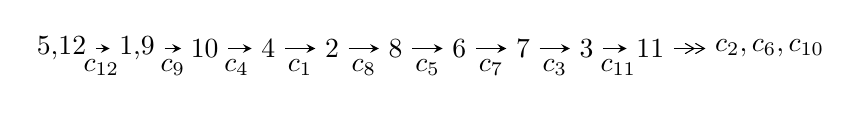
\begin{tikzpicture}[x=23pt, y=7pt]
	% node
	\node (A0) at (-1/8, 0) {5,12};
	\node (A1) at (17/16, 0) {1,9};
	\node (A2) at (17/8, 0) {10};
	\node (A3) at (25/8, 0) {4};
	\node (A4) at (33/8, 0) {2};
	\node (A5) at (41/8, 0) {8};
	\node (A6) at (49/8, 0) {6};
	\node (A7) at (57/8, 0) {7};
	\node (A8) at (65/8, 0) {3};
	\node (A9) at (73/8, 0) {11};
	\node (C1) at (1/2, -1) {$c_{12}$};
	\node (C2) at (13/8, -1) {$c_{9}$};
	\node (C3) at (21/8, -1) {$c_{4}$};
	\node (C4) at (29/8, -1) {$c_{1}$};
	\node (C5) at (37/8, -1) {$c_{8}$};
	\node (C6) at (45/8, -1) {$c_{5}$};
	\node (C7) at (53/8, -1) {$c_{7}$};
	\node (C8) at (61/8, -1) {$c_{3}$};
	\node (C9) at (69/8, -1) {$c_{11}$};
	\node (A10) at (11, 0) {$c_{2},c_{6},c_{10}$};

	% edge
	\draw[->,>=stealth]	
	(A0) edge (A1) (A1) edge (A2) (A2) edge (A3) (A3) edge (A4) (A4) edge (A5) (A5) edge (A6) (A6) edge (A7) (A7) edge (A8) (A8) edge (A9) ;
	\draw[->>,>={angle 60}]	
	(A9) edge (A10);
\end{tikzpicture} \\ 

\end{tabular} \\

\footnotetext{
The image of knot diagram is generated by the software ``\textbf{Draw programme}" developed by Andrew Bartholomew(\url{http://www.layer8.co.uk/maths/draw/index.htm\#Running-draw}), where we modified some parts for our purpose(\url{https://github.com/CATsTAILs/LinksPainter}).
}\phantom \\ \newline 
\centering \textbf{Ideals for irreducible components\footnotemark of $X_{\text{par}}$} 
 
\begin{align*}
I^u_{1}&=\langle 
-5.34907\times10^{25} u^{25}-1.80642\times10^{26} u^{24}+\cdots+7.92164\times10^{25} b+4.11760\times10^{26},\\
\phantom{I^u_{1}}&\phantom{= \langle  }3.95167\times10^{23} u^{25}+1.51546\times10^{24} u^{24}+\cdots+2.64055\times10^{25} a-6.82923\times10^{25},\;u^{26}+3 u^{25}+\cdots-15 u+3\rangle \\
I^u_{2}&=\langle 
2.73334\times10^{2858} u^{227}-1.92123\times10^{2858} u^{226}+\cdots+4.27537\times10^{2861} b+2.16549\times10^{2863},\\
\phantom{I^u_{2}}&\phantom{= \langle  }4.43607\times10^{2844} u^{227}+8.55713\times10^{2844} u^{226}+\cdots+8.30905\times10^{2847} a+4.47338\times10^{2849},\\
\phantom{I^u_{2}}&\phantom{= \langle  }u^{228}-2 u^{227}+\cdots-120069 u+8487\rangle \\
I^u_{3}&=\langle 
1.77876\times10^{199} u^{59}-4.11117\times10^{199} u^{58}+\cdots+4.10975\times10^{201} b-1.03369\times10^{201},\\
\phantom{I^u_{3}}&\phantom{= \langle  }-1.12963\times10^{195} u^{59}+3.04187\times10^{195} u^{58}+\cdots+3.32182\times10^{196} a+1.29221\times10^{197},\\
\phantom{I^u_{3}}&\phantom{= \langle  }u^{60}-3 u^{59}+\cdots-405 u+81\rangle \\
I^u_{4}&=\langle 
- u^5-3 u^4-4 u^3-3 u^2+b- u-1,\;- u^4-2 u^3-3 u^2+a-2 u-1,\;u^6+3 u^5+5 u^4+4 u^3+2 u^2+u+1\rangle \\
\\
\end{align*}
\raggedright * 4 irreducible components of $\dim_{\mathbb{C}}=0$, with total 320 representations.\\
\footnotetext{All coefficients of polynomials are rational numbers. But the coefficients are sometimes approximated in decimal forms when there is not enough margin.}
\newpage
\renewcommand{\arraystretch}{1}
\centering \section*{I. $I^u_{1}= \langle -5.35\times10^{25} u^{25}-1.81\times10^{26} u^{24}+\cdots+7.92\times10^{25} b+4.12\times10^{26},\;3.95\times10^{23} u^{25}+1.52\times10^{24} u^{24}+\cdots+2.64\times10^{25} a-6.83\times10^{25},\;u^{26}+3 u^{25}+\cdots-15 u+3 \rangle$}
\flushleft \textbf{(i) Arc colorings}\\
\begin{tabular}{m{7pt} m{180pt} m{7pt} m{180pt} }
\flushright $a_{5}=$&$\begin{pmatrix}0\\u\end{pmatrix}$ \\
\flushright $a_{12}=$&$\begin{pmatrix}1\\0\end{pmatrix}$ \\
\flushright $a_{1}=$&$\begin{pmatrix}1\\- u^2\end{pmatrix}$ \\
\flushright $a_{9}=$&$\begin{pmatrix}-0.0149653 u^{25}-0.0573920 u^{24}+\cdots-5.13455 u+2.58629\\0.675248 u^{25}+2.28036 u^{24}+\cdots+14.2808 u-5.19791\end{pmatrix}$ \\
\flushright $a_{10}=$&$\begin{pmatrix}-0.632801 u^{25}-2.22531 u^{24}+\cdots-19.2728 u+7.74671\\0.825829 u^{25}+2.74001 u^{24}+\cdots+17.1435 u-6.14114\end{pmatrix}$ \\
\flushright $a_{4}=$&$\begin{pmatrix}-0.674011 u^{25}-2.06149 u^{24}+\cdots-0.724059 u+0.371443\\0.0748759 u^{25}+0.392514 u^{24}+\cdots+2.78632 u-1.21956\end{pmatrix}$ \\
\flushright $a_{2}=$&$\begin{pmatrix}-0.757263 u^{25}-2.08651 u^{24}+\cdots-10.3107 u+2.23996\\0.267117 u^{25}+0.978083 u^{24}+\cdots+2.56900 u-2.07064\end{pmatrix}$ \\
\flushright $a_{8}=$&$\begin{pmatrix}-0.690213 u^{25}-2.33776 u^{24}+\cdots-19.4154 u+7.78420\\0.675248 u^{25}+2.28036 u^{24}+\cdots+14.2808 u-5.19791\end{pmatrix}$ \\
\flushright $a_{6}=$&$\begin{pmatrix}-0.851189 u^{25}-2.96069 u^{24}+\cdots-6.06101 u+2.28294\\0.102302 u^{25}+0.506686 u^{24}+\cdots+4.55063 u-0.691938\end{pmatrix}$ \\
\flushright $a_{7}=$&$\begin{pmatrix}-0.424070 u^{25}-1.10116 u^{24}+\cdots-17.7829 u+3.92612\\0.166509 u^{25}+0.680241 u^{24}+\cdots+0.997296 u+0.529442\end{pmatrix}$ \\
\flushright $a_{3}=$&$\begin{pmatrix}0.815413 u^{25}+2.85812 u^{24}+\cdots+23.5628 u-11.7902\\-1.40196 u^{25}-4.61527 u^{24}+\cdots-26.5088 u+11.0509\end{pmatrix}$ \\
\flushright $a_{11}=$&$\begin{pmatrix}-0.547726 u^{25}-1.21606 u^{24}+\cdots+8.21515 u-3.50603\\-0.407127 u^{25}-1.15717 u^{24}+\cdots-10.4849 u+2.55357\end{pmatrix}$\\&\end{tabular}
\flushleft \textbf{(ii) Obstruction class $= -1$}\\~\\
\flushleft \textbf{(iii) Cusp Shapes $= \frac{1260977761418218210095504584}{237649321085197816953007317} u^{25}+\frac{1395857718298382707824957472}{79216440361732605651002439} u^{24}+\cdots+\frac{36059835826067669335416717074}{237649321085197816953007317} u-\frac{4085664600030892994473000376}{79216440361732605651002439}$}\\~\\
\newpage\renewcommand{\arraystretch}{1}
\flushleft \textbf{(iv) u-Polynomials at the component}\newline \\
\begin{tabular}{m{50pt}|m{274pt}}
Crossings & \hspace{64pt}u-Polynomials at each crossing \\
\hline $$\begin{aligned}c_{1},c_{7}\end{aligned}$$&$\begin{aligned}
&u^{26}- u^{25}+\cdots+21 u+7
\end{aligned}$\\
\hline $$\begin{aligned}c_{2},c_{8}\end{aligned}$$&$\begin{aligned}
&3(3 u^{26}-3 u^{25}+\cdots- u+1)
\end{aligned}$\\
\hline $$\begin{aligned}c_{3},c_{9}\end{aligned}$$&$\begin{aligned}
&3(3 u^{26}+3 u^{25}+\cdots+u+1)
\end{aligned}$\\
\hline $$\begin{aligned}c_{4},c_{10}\end{aligned}$$&$\begin{aligned}
&u^{26}+3 u^{25}+\cdots-15 u+3
\end{aligned}$\\
\hline $$\begin{aligned}c_{5},c_{11}\end{aligned}$$&$\begin{aligned}
&u^{26}+u^{25}+\cdots-21 u+7
\end{aligned}$\\
\hline $$\begin{aligned}c_{6},c_{12}\end{aligned}$$&$\begin{aligned}
&u^{26}-3 u^{25}+\cdots+15 u+3
\end{aligned}$\\
\hline
\end{tabular}\\~\\
\newpage\renewcommand{\arraystretch}{1}
\flushleft \textbf{(v) Riley Polynomials at the component}\newline \\
\begin{tabular}{m{50pt}|m{274pt}}
Crossings & \hspace{64pt}Riley Polynomials at each crossing \\
\hline $$\begin{aligned}c_{1},c_{5},c_{7}\\c_{11}\end{aligned}$$&$\begin{aligned}
&y^{26}+15 y^{25}+\cdots+777 y+49
\end{aligned}$\\
\hline $$\begin{aligned}c_{2},c_{3},c_{8}\\c_{9}\end{aligned}$$&$\begin{aligned}
&9(9 y^{26}+123 y^{25}+\cdots-3 y+1)
\end{aligned}$\\
\hline $$\begin{aligned}c_{4},c_{6},c_{10}\\c_{12}\end{aligned}$$&$\begin{aligned}
&y^{26}+3 y^{25}+\cdots-39 y+9
\end{aligned}$\\
\hline
\end{tabular}\\~\\
\newpage\flushleft \textbf{(vi) Complex Volumes and Cusp Shapes}
$$\begin{array}{c|c|c}  
\text{Solutions to }I^u_{1}& \I (\text{vol} + \sqrt{-1}CS) & \text{Cusp shape}\\
 \hline 
\begin{aligned}
u &= \phantom{-}0.845489 + 0.535083 I \\
a &= \phantom{-}0.02844 + 1.51551 I \\
b &= \phantom{-}0.335856 + 0.179407 I\end{aligned}
 & \phantom{-}3.75175 + 7.29916 I & \phantom{-}7.10463 - 6.60908 I \\ \hline\begin{aligned}
u &= \phantom{-}0.845489 - 0.535083 I \\
a &= \phantom{-}0.02844 - 1.51551 I \\
b &= \phantom{-}0.335856 - 0.179407 I\end{aligned}
 & \phantom{-}3.75175 - 7.29916 I & \phantom{-}7.10463 + 6.60908 I \\ \hline\begin{aligned}
u &= -0.412083 + 0.907598 I \\
a &= -1.229110 + 0.268720 I \\
b &= -0.327018 - 0.255373 I\end{aligned}
 & -1.031450 - 0.731362 I & -5.81274 + 5.12436 I \\ \hline\begin{aligned}
u &= -0.412083 - 0.907598 I \\
a &= -1.229110 - 0.268720 I \\
b &= -0.327018 + 0.255373 I\end{aligned}
 & -1.031450 + 0.731362 I & -5.81274 - 5.12436 I \\ \hline\begin{aligned}
u &= \phantom{-}0.815740 + 0.766504 I \\
a &= \phantom{-}0.037856 + 1.304310 I \\
b &= \phantom{-}0.95346 + 1.24193 I\end{aligned}
 & \phantom{-}3.90122 + 10.59870 I & \phantom{-}3.57222 - 11.00535 I \\ \hline\begin{aligned}
u &= \phantom{-}0.815740 - 0.766504 I \\
a &= \phantom{-}0.037856 - 1.304310 I \\
b &= \phantom{-}0.95346 - 1.24193 I\end{aligned}
 & \phantom{-}3.90122 - 10.59870 I & \phantom{-}3.57222 + 11.00535 I \\ \hline\begin{aligned}
u &= \phantom{-}0.262607 + 1.226280 I \\
a &= -0.776479 + 0.169761 I \\
b &= -0.677732 + 0.488296 I\end{aligned}
 & \phantom{-}1.031450 - 0.731362 I & \phantom{-}5.81274 + 5.12436 I \\ \hline\begin{aligned}
u &= \phantom{-}0.262607 - 1.226280 I \\
a &= -0.776479 - 0.169761 I \\
b &= -0.677732 - 0.488296 I\end{aligned}
 & \phantom{-}1.031450 + 0.731362 I & \phantom{-}5.81274 - 5.12436 I \\ \hline\begin{aligned}
u &= \phantom{-}0.483028 + 0.515672 I \\
a &= -0.11814 - 2.27233 I \\
b &= -0.207260 - 0.904960 I\end{aligned}
 & \phantom{-}1.45995 + 7.35605 I & -7.17269 - 6.50998 I \\ \hline\begin{aligned}
u &= \phantom{-}0.483028 - 0.515672 I \\
a &= -0.11814 + 2.27233 I \\
b &= -0.207260 + 0.904960 I\end{aligned}
 & \phantom{-}1.45995 - 7.35605 I & -7.17269 + 6.50998 I\\
 \hline 
 \end{array}$$\newpage$$\begin{array}{c|c|c}  
\text{Solutions to }I^u_{1}& \I (\text{vol} + \sqrt{-1}CS) & \text{Cusp shape}\\
 \hline 
\begin{aligned}
u &= -0.167410 + 0.663095 I \\
a &= \phantom{-}1.65128 + 2.17905 I \\
b &= -0.329021 + 0.860688 I\end{aligned}
 & -2.74535 - 5.73210 I & -12.7377 + 11.1594 I \\ \hline\begin{aligned}
u &= -0.167410 - 0.663095 I \\
a &= \phantom{-}1.65128 - 2.17905 I \\
b &= -0.329021 - 0.860688 I\end{aligned}
 & -2.74535 + 5.73210 I & -12.7377 - 11.1594 I \\ \hline\begin{aligned}
u &= -0.291479 + 0.576161 I \\
a &= -0.592442 + 0.805613 I \\
b &= -0.208461 + 0.489857 I\end{aligned}
 & \phantom{-0.000000 } -1.28045 I & \phantom{-0.000000 -}0. + 5.59729 I \\ \hline\begin{aligned}
u &= -0.291479 - 0.576161 I \\
a &= -0.592442 - 0.805613 I \\
b &= -0.208461 - 0.489857 I\end{aligned}
 & \phantom{-0.000000 -}1.28045 I & \phantom{-0.000000 } 0. - 5.59729 I \\ \hline\begin{aligned}
u &= -0.96888 + 1.09299 I \\
a &= \phantom{-}0.022234 - 0.766044 I \\
b &= \phantom{-}0.67467 - 1.39088 I\end{aligned}
 & -3.90122 - 10.59870 I & -3.57222 + 11.00535 I \\ \hline\begin{aligned}
u &= -0.96888 - 1.09299 I \\
a &= \phantom{-}0.022234 + 0.766044 I \\
b &= \phantom{-}0.67467 + 1.39088 I\end{aligned}
 & -3.90122 + 10.59870 I & -3.57222 - 11.00535 I \\ \hline\begin{aligned}
u &= -0.78688 + 1.29657 I \\
a &= \phantom{-}0.012380 - 0.659611 I \\
b &= \phantom{-}1.023210 - 0.854597 I\end{aligned}
 & -3.75175 - 7.29916 I & -7.10463 + 6.60908 I \\ \hline\begin{aligned}
u &= -0.78688 - 1.29657 I \\
a &= \phantom{-}0.012380 + 0.659611 I \\
b &= \phantom{-}1.023210 + 0.854597 I\end{aligned}
 & -3.75175 + 7.29916 I & -7.10463 - 6.60908 I \\ \hline\begin{aligned}
u &= -1.03954 + 1.20307 I \\
a &= -0.145069 + 0.989422 I \\
b &= -1.26401 + 1.10023 I\end{aligned}
 & \phantom{-0.000000 } -23.4387 I & \phantom{-0.000000 -}0. + 11.88508 I \\ \hline\begin{aligned}
u &= -1.03954 - 1.20307 I \\
a &= -0.145069 - 0.989422 I \\
b &= -1.26401 - 1.10023 I\end{aligned}
 & \phantom{-0.000000 -}23.4387 I & \phantom{-0.000000 } 0. - 11.88508 I\\
 \hline 
 \end{array}$$\newpage$$\begin{array}{c|c|c}  
\text{Solutions to }I^u_{1}& \I (\text{vol} + \sqrt{-1}CS) & \text{Cusp shape}\\
 \hline 
\begin{aligned}
u &= \phantom{-}1.11471 + 1.15852 I \\
a &= -0.022818 - 0.438890 I \\
b &= -0.928596 - 0.889733 I\end{aligned}
 & -1.45995 + 7.35605 I & \phantom{-}7.17269 - 6.50998 I \\ \hline\begin{aligned}
u &= \phantom{-}1.11471 - 1.15852 I \\
a &= -0.022818 + 0.438890 I \\
b &= -0.928596 + 0.889733 I\end{aligned}
 & -1.45995 - 7.35605 I & \phantom{-}7.17269 + 6.50998 I \\ \hline\begin{aligned}
u &= \phantom{-}0.366048 + 0.079011 I \\
a &= \phantom{-}0.910967 - 0.412479 I \\
b &= -0.07012 + 2.08604 I\end{aligned}
 & \phantom{-0.000000 } -3.95888 I & \phantom{-0.000000 -}0. + 19.3379 I \\ \hline\begin{aligned}
u &= \phantom{-}0.366048 - 0.079011 I \\
a &= \phantom{-}0.910967 + 0.412479 I \\
b &= -0.07012 - 2.08604 I\end{aligned}
 & \phantom{-0.000000 -}3.95888 I & \phantom{-0.000000 } 0. - 19.3379 I \\ \hline\begin{aligned}
u &= -1.72136 + 0.73016 I \\
a &= \phantom{-}0.220907 - 0.291513 I \\
b &= \phantom{-}0.525012 + 0.402973 I\end{aligned}
 & \phantom{-}2.74535 + 5.73210 I & \phantom{-}12.7377 - 11.1594 I \\ \hline\begin{aligned}
u &= -1.72136 - 0.73016 I \\
a &= \phantom{-}0.220907 + 0.291513 I \\
b &= \phantom{-}0.525012 - 0.402973 I\end{aligned}
 & \phantom{-}2.74535 - 5.73210 I & \phantom{-}12.7377 + 11.1594 I\\
 \hline 
 \end{array}$$\newpage\newpage\renewcommand{\arraystretch}{1}
\centering \section*{II. $I^u_{2}= \langle 2.73\times10^{2858} u^{227}-1.92\times10^{2858} u^{226}+\cdots+4.28\times10^{2861} b+2.17\times10^{2863},\;4.44\times10^{2844} u^{227}+8.56\times10^{2844} u^{226}+\cdots+8.31\times10^{2847} a+4.47\times10^{2849},\;u^{228}-2 u^{227}+\cdots-120069 u+8487 \rangle$}
\flushleft \textbf{(i) Arc colorings}\\
\begin{tabular}{m{7pt} m{180pt} m{7pt} m{180pt} }
\flushright $a_{5}=$&$\begin{pmatrix}0\\u\end{pmatrix}$ \\
\flushright $a_{12}=$&$\begin{pmatrix}1\\0\end{pmatrix}$ \\
\flushright $a_{1}=$&$\begin{pmatrix}1\\- u^2\end{pmatrix}$ \\
\flushright $a_{9}=$&$\begin{pmatrix}-0.000533884 u^{227}-0.00102986 u^{226}+\cdots+509.800 u-53.8374\\-0.000639322 u^{227}+0.000449372 u^{226}+\cdots+665.496 u-50.6504\end{pmatrix}$ \\
\flushright $a_{10}=$&$\begin{pmatrix}0.000973408 u^{227}-0.00355423 u^{226}+\cdots+91.6330 u-20.9896\\-0.000312050 u^{227}-0.0000481389 u^{226}+\cdots+619.429 u-46.4900\end{pmatrix}$ \\
\flushright $a_{4}=$&$\begin{pmatrix}-0.00260219 u^{227}+0.00541797 u^{226}+\cdots-591.763 u+39.6752\\-0.000294906 u^{227}-0.000314458 u^{226}+\cdots+350.080 u-26.3569\end{pmatrix}$ \\
\flushright $a_{2}=$&$\begin{pmatrix}0.00943454 u^{227}-0.0189153 u^{226}+\cdots+1354.50 u-84.5624\\0.00101777 u^{227}-0.00171219 u^{226}+\cdots-78.1751 u+8.76891\end{pmatrix}$ \\
\flushright $a_{8}=$&$\begin{pmatrix}0.000105438 u^{227}-0.00147923 u^{226}+\cdots-155.696 u-3.18704\\-0.000639322 u^{227}+0.000449372 u^{226}+\cdots+665.496 u-50.6504\end{pmatrix}$ \\
\flushright $a_{6}=$&$\begin{pmatrix}-0.00317145 u^{227}+0.00769773 u^{226}+\cdots-1569.89 u+108.053\\0.000864162 u^{227}-0.00196531 u^{226}+\cdots+630.046 u-42.0209\end{pmatrix}$ \\
\flushright $a_{7}=$&$\begin{pmatrix}-0.00844623 u^{227}+0.0132865 u^{226}+\cdots+77.7048 u-39.3309\\0.000578702 u^{227}-0.00216850 u^{226}+\cdots+752.583 u-48.3559\end{pmatrix}$ \\
\flushright $a_{3}=$&$\begin{pmatrix}0.00876827 u^{227}-0.0152721 u^{226}+\cdots-650.077 u+79.1653\\-0.00279035 u^{227}+0.00568240 u^{226}+\cdots-389.402 u+6.90679\end{pmatrix}$ \\
\flushright $a_{11}=$&$\begin{pmatrix}0.00684100 u^{227}-0.0134311 u^{226}+\cdots+611.474 u-13.4745\\0.00135278 u^{227}-0.00106211 u^{226}+\cdots-388.490 u+29.0289\end{pmatrix}$\\&\end{tabular}
\flushleft \textbf{(ii) Obstruction class $= -1$}\\~\\
\flushleft \textbf{(iii) Cusp Shapes $= 0.00480003 u^{227}-0.00745917 u^{226}+\cdots-106.584 u-13.9909$}\\~\\
\newpage\renewcommand{\arraystretch}{1}
\flushleft \textbf{(iv) u-Polynomials at the component}\newline \\
\begin{tabular}{m{50pt}|m{274pt}}
Crossings & \hspace{64pt}u-Polynomials at each crossing \\
\hline $$\begin{aligned}c_{1},c_{7}\end{aligned}$$&$\begin{aligned}
&u^{228}+8 u^{227}+\cdots-11192067647 u+984049733
\end{aligned}$\\
\hline $$\begin{aligned}c_{2},c_{8}\end{aligned}$$&$\begin{aligned}
&9(9 u^{228}-54 u^{227}+\cdots-9395 u+1619)
\end{aligned}$\\
\hline $$\begin{aligned}c_{3},c_{9}\end{aligned}$$&$\begin{aligned}
&9(9 u^{228}+54 u^{227}+\cdots+9395 u+1619)
\end{aligned}$\\
\hline $$\begin{aligned}c_{4},c_{10}\end{aligned}$$&$\begin{aligned}
&u^{228}-2 u^{227}+\cdots-120069 u+8487
\end{aligned}$\\
\hline $$\begin{aligned}c_{5},c_{11}\end{aligned}$$&$\begin{aligned}
&u^{228}-8 u^{227}+\cdots+11192067647 u+984049733
\end{aligned}$\\
\hline $$\begin{aligned}c_{6},c_{12}\end{aligned}$$&$\begin{aligned}
&u^{228}+2 u^{227}+\cdots+120069 u+8487
\end{aligned}$\\
\hline
\end{tabular}\\~\\
\newpage\renewcommand{\arraystretch}{1}
\flushleft \textbf{(v) Riley Polynomials at the component}\newline \\
\begin{tabular}{m{50pt}|m{274pt}}
Crossings & \hspace{64pt}Riley Polynomials at each crossing \\
\hline $$\begin{aligned}c_{1},c_{5},c_{7}\\c_{11}\end{aligned}$$&$\begin{aligned}
&y^{228}+20 y^{227}+\cdots+4.78\times10^{19} y+9.68\times10^{17}
\end{aligned}$\\
\hline $$\begin{aligned}c_{2},c_{3},c_{8}\\c_{9}\end{aligned}$$&$\begin{aligned}
&81(81 y^{228}+2052 y^{227}+\cdots+8.92055\times10^{7} y+2621161)
\end{aligned}$\\
\hline $$\begin{aligned}c_{4},c_{6},c_{10}\\c_{12}\end{aligned}$$&$\begin{aligned}
&y^{228}+12 y^{227}+\cdots+6749419149 y+72029169
\end{aligned}$\\
\hline
\end{tabular}\\~\\
\newpage\flushleft \textbf{(vi) Complex Volumes and Cusp Shapes}
$$\begin{array}{c|c|c}  
\text{Solutions to }I^u_{2}& \I (\text{vol} + \sqrt{-1}CS) & \text{Cusp shape}\\
 \hline 
\begin{aligned}
u &= -0.472631 + 0.876801 I \\
a &= -0.270968 + 1.060490 I \\
b &= \phantom{-}0.104155 + 1.397710 I\end{aligned}
 & -0.17902 - 4.15433 I & \phantom{-0.000000 } 0 \\ \hline\begin{aligned}
u &= -0.472631 - 0.876801 I \\
a &= -0.270968 - 1.060490 I \\
b &= \phantom{-}0.104155 - 1.397710 I\end{aligned}
 & -0.17902 + 4.15433 I & \phantom{-0.000000 } 0 \\ \hline\begin{aligned}
u &= \phantom{-}0.700933 + 0.696420 I \\
a &= \phantom{-}0.16116 - 1.40722 I \\
b &= -1.09140 - 1.19241 I\end{aligned}
 & \phantom{-}2.61654 + 5.18045 I & \phantom{-0.000000 } 0 \\ \hline\begin{aligned}
u &= \phantom{-}0.700933 - 0.696420 I \\
a &= \phantom{-}0.16116 + 1.40722 I \\
b &= -1.09140 + 1.19241 I\end{aligned}
 & \phantom{-}2.61654 - 5.18045 I & \phantom{-0.000000 } 0 \\ \hline\begin{aligned}
u &= -0.887697 + 0.424622 I \\
a &= -0.244267 + 0.750770 I \\
b &= -1.07432 + 1.25389 I\end{aligned}
 & \phantom{-}0.71894 - 5.15211 I & \phantom{-0.000000 } 0 \\ \hline\begin{aligned}
u &= -0.887697 - 0.424622 I \\
a &= -0.244267 - 0.750770 I \\
b &= -1.07432 - 1.25389 I\end{aligned}
 & \phantom{-}0.71894 + 5.15211 I & \phantom{-0.000000 } 0 \\ \hline\begin{aligned}
u &= \phantom{-}0.614351 + 0.767456 I \\
a &= -0.14177 - 1.76236 I \\
b &= -0.91137 - 1.10218 I\end{aligned}
 & \phantom{-}1.72572 + 7.49064 I & \phantom{-0.000000 } 0 \\ \hline\begin{aligned}
u &= \phantom{-}0.614351 - 0.767456 I \\
a &= -0.14177 + 1.76236 I \\
b &= -0.91137 + 1.10218 I\end{aligned}
 & \phantom{-}1.72572 - 7.49064 I & \phantom{-0.000000 } 0 \\ \hline\begin{aligned}
u &= \phantom{-}0.405452 + 0.887384 I \\
a &= \phantom{-}0.458615 - 0.144400 I \\
b &= \phantom{-}1.196280 - 0.210695 I\end{aligned}
 & -1.17272 - 3.22672 I & \phantom{-0.000000 } 0 \\ \hline\begin{aligned}
u &= \phantom{-}0.405452 - 0.887384 I \\
a &= \phantom{-}0.458615 + 0.144400 I \\
b &= \phantom{-}1.196280 + 0.210695 I\end{aligned}
 & -1.17272 + 3.22672 I & \phantom{-0.000000 } 0\\
 \hline 
 \end{array}$$\newpage$$\begin{array}{c|c|c}  
\text{Solutions to }I^u_{2}& \I (\text{vol} + \sqrt{-1}CS) & \text{Cusp shape}\\
 \hline 
\begin{aligned}
u &= -0.437652 + 0.926858 I \\
a &= -0.111817 - 0.254381 I \\
b &= -1.227690 - 0.425841 I\end{aligned}
 & -2.15015 - 8.23570 I & \phantom{-0.000000 } 0 \\ \hline\begin{aligned}
u &= -0.437652 - 0.926858 I \\
a &= -0.111817 + 0.254381 I \\
b &= -1.227690 + 0.425841 I\end{aligned}
 & -2.15015 + 8.23570 I & \phantom{-0.000000 } 0 \\ \hline\begin{aligned}
u &= -0.563747 + 0.865746 I \\
a &= -0.47100 + 1.56851 I \\
b &= -1.12449 + 1.24533 I\end{aligned}
 & \phantom{-}2.77141 - 2.42490 I & \phantom{-0.000000 } 0 \\ \hline\begin{aligned}
u &= -0.563747 - 0.865746 I \\
a &= -0.47100 - 1.56851 I \\
b &= -1.12449 - 1.24533 I\end{aligned}
 & \phantom{-}2.77141 + 2.42490 I & \phantom{-0.000000 } 0 \\ \hline\begin{aligned}
u &= \phantom{-}0.303668 + 0.909247 I \\
a &= -0.144875 + 0.536056 I \\
b &= \phantom{-}0.974296 + 0.848762 I\end{aligned}
 & -4.07623 - 0.75664 I & \phantom{-0.000000 } 0 \\ \hline\begin{aligned}
u &= \phantom{-}0.303668 - 0.909247 I \\
a &= -0.144875 - 0.536056 I \\
b &= \phantom{-}0.974296 - 0.848762 I\end{aligned}
 & -4.07623 + 0.75664 I & \phantom{-0.000000 } 0 \\ \hline\begin{aligned}
u &= \phantom{-}0.808370 + 0.673531 I \\
a &= \phantom{-}0.09053 + 1.41138 I \\
b &= \phantom{-}1.255900 + 0.646328 I\end{aligned}
 & \phantom{-}4.14980 - 4.96562 I & \phantom{-0.000000 } 0 \\ \hline\begin{aligned}
u &= \phantom{-}0.808370 - 0.673531 I \\
a &= \phantom{-}0.09053 - 1.41138 I \\
b &= \phantom{-}1.255900 - 0.646328 I\end{aligned}
 & \phantom{-}4.14980 + 4.96562 I & \phantom{-0.000000 } 0 \\ \hline\begin{aligned}
u &= -0.025731 + 0.947303 I \\
a &= -1.56751 - 0.39571 I \\
b &= -0.208138 - 0.172320 I\end{aligned}
 & -2.91798 + 1.45918 I & \phantom{-0.000000 } 0 \\ \hline\begin{aligned}
u &= -0.025731 - 0.947303 I \\
a &= -1.56751 + 0.39571 I \\
b &= -0.208138 + 0.172320 I\end{aligned}
 & -2.91798 - 1.45918 I & \phantom{-0.000000 } 0\\
 \hline 
 \end{array}$$\newpage$$\begin{array}{c|c|c}  
\text{Solutions to }I^u_{2}& \I (\text{vol} + \sqrt{-1}CS) & \text{Cusp shape}\\
 \hline 
\begin{aligned}
u &= -0.948463 + 0.456251 I \\
a &= -0.176635 - 1.187010 I \\
b &= \phantom{-}0.574232 - 0.241509 I\end{aligned}
 & \phantom{-}4.07623 - 0.75664 I & \phantom{-0.000000 } 0 \\ \hline\begin{aligned}
u &= -0.948463 - 0.456251 I \\
a &= -0.176635 + 1.187010 I \\
b &= \phantom{-}0.574232 + 0.241509 I\end{aligned}
 & \phantom{-}4.07623 + 0.75664 I & \phantom{-0.000000 } 0 \\ \hline\begin{aligned}
u &= -0.077732 + 0.942885 I \\
a &= -0.966354 + 0.671156 I \\
b &= \phantom{-}0.018451 + 0.708666 I\end{aligned}
 & -1.53101 - 2.78696 I & \phantom{-0.000000 } 0 \\ \hline\begin{aligned}
u &= -0.077732 - 0.942885 I \\
a &= -0.966354 - 0.671156 I \\
b &= \phantom{-}0.018451 - 0.708666 I\end{aligned}
 & -1.53101 + 2.78696 I & \phantom{-0.000000 } 0 \\ \hline\begin{aligned}
u &= \phantom{-}0.903835 + 0.275047 I \\
a &= \phantom{-}0.021923 - 0.746122 I \\
b &= -1.054210 - 0.744065 I\end{aligned}
 & \phantom{-}4.18899 + 2.61263 I & \phantom{-0.000000 } 0 \\ \hline\begin{aligned}
u &= \phantom{-}0.903835 - 0.275047 I \\
a &= \phantom{-}0.021923 + 0.746122 I \\
b &= -1.054210 + 0.744065 I\end{aligned}
 & \phantom{-}4.18899 - 2.61263 I & \phantom{-0.000000 } 0 \\ \hline\begin{aligned}
u &= \phantom{-}0.308872 + 0.865220 I \\
a &= -0.889294 + 0.058440 I \\
b &= -0.991086 + 0.494295 I\end{aligned}
 & \phantom{-}1.17272 - 3.22672 I & \phantom{-0.000000 } 0 \\ \hline\begin{aligned}
u &= \phantom{-}0.308872 - 0.865220 I \\
a &= -0.889294 - 0.058440 I \\
b &= -0.991086 - 0.494295 I\end{aligned}
 & \phantom{-}1.17272 + 3.22672 I & \phantom{-0.000000 } 0 \\ \hline\begin{aligned}
u &= \phantom{-}0.626212 + 0.671141 I \\
a &= \phantom{-}1.298530 + 0.548758 I \\
b &= -0.051458 - 0.690948 I\end{aligned}
 & -2.61654 + 5.18045 I & \phantom{-0.000000 } 0 \\ \hline\begin{aligned}
u &= \phantom{-}0.626212 - 0.671141 I \\
a &= \phantom{-}1.298530 - 0.548758 I \\
b &= -0.051458 + 0.690948 I\end{aligned}
 & -2.61654 - 5.18045 I & \phantom{-0.000000 } 0\\
 \hline 
 \end{array}$$\newpage$$\begin{array}{c|c|c}  
\text{Solutions to }I^u_{2}& \I (\text{vol} + \sqrt{-1}CS) & \text{Cusp shape}\\
 \hline 
\begin{aligned}
u &= -0.801773 + 0.738807 I \\
a &= -0.226171 + 0.885169 I \\
b &= -1.13088 + 1.04390 I\end{aligned}
 & \phantom{-}0.17902 - 4.15433 I & \phantom{-0.000000 } 0 \\ \hline\begin{aligned}
u &= -0.801773 - 0.738807 I \\
a &= -0.226171 - 0.885169 I \\
b &= -1.13088 - 1.04390 I\end{aligned}
 & \phantom{-}0.17902 + 4.15433 I & \phantom{-0.000000 } 0 \\ \hline\begin{aligned}
u &= -0.698841 + 0.580141 I \\
a &= -0.083419 - 1.356350 I \\
b &= \phantom{-}0.402780 - 1.316530 I\end{aligned}
 & \phantom{-}3.12185\phantom{ +0.000000I} & \phantom{-0.000000 } 0 \\ \hline\begin{aligned}
u &= -0.698841 - 0.580141 I \\
a &= -0.083419 + 1.356350 I \\
b &= \phantom{-}0.402780 + 1.316530 I\end{aligned}
 & \phantom{-}3.12185\phantom{ +0.000000I} & \phantom{-0.000000 } 0 \\ \hline\begin{aligned}
u &= \phantom{-}0.819062 + 0.385256 I \\
a &= \phantom{-}0.147418 + 0.730746 I \\
b &= \phantom{-}1.32930 + 1.44019 I\end{aligned}
 & \phantom{-}1.35038 + 13.87800 I & \phantom{-0.000000 } 0 \\ \hline\begin{aligned}
u &= \phantom{-}0.819062 - 0.385256 I \\
a &= \phantom{-}0.147418 - 0.730746 I \\
b &= \phantom{-}1.32930 - 1.44019 I\end{aligned}
 & \phantom{-}1.35038 - 13.87800 I & \phantom{-0.000000 } 0 \\ \hline\begin{aligned}
u &= \phantom{-}0.803943 + 0.408919 I \\
a &= -0.073299 - 0.595618 I \\
b &= -1.33268 - 1.32831 I\end{aligned}
 & \phantom{-}2.04342 + 5.79434 I & \phantom{-0.000000 } 0 \\ \hline\begin{aligned}
u &= \phantom{-}0.803943 - 0.408919 I \\
a &= -0.073299 + 0.595618 I \\
b &= -1.33268 + 1.32831 I\end{aligned}
 & \phantom{-}2.04342 - 5.79434 I & \phantom{-0.000000 } 0 \\ \hline\begin{aligned}
u &= -0.557707 + 0.963331 I \\
a &= -0.698086 + 0.484838 I \\
b &= -0.970114 + 0.257695 I\end{aligned}
 & \phantom{-}1.53101 - 2.78696 I & \phantom{-0.000000 } 0 \\ \hline\begin{aligned}
u &= -0.557707 - 0.963331 I \\
a &= -0.698086 - 0.484838 I \\
b &= -0.970114 - 0.257695 I\end{aligned}
 & \phantom{-}1.53101 + 2.78696 I & \phantom{-0.000000 } 0\\
 \hline 
 \end{array}$$\newpage$$\begin{array}{c|c|c}  
\text{Solutions to }I^u_{2}& \I (\text{vol} + \sqrt{-1}CS) & \text{Cusp shape}\\
 \hline 
\begin{aligned}
u &= -1.108000 + 0.112943 I \\
a &= -1.153980 + 0.300686 I \\
b &= \phantom{-}0.618423 - 0.131290 I\end{aligned}
 & \phantom{-}2.60879 + 0.44068 I & \phantom{-0.000000 } 0 \\ \hline\begin{aligned}
u &= -1.108000 - 0.112943 I \\
a &= -1.153980 - 0.300686 I \\
b &= \phantom{-}0.618423 + 0.131290 I\end{aligned}
 & \phantom{-}2.60879 - 0.44068 I & \phantom{-0.000000 } 0 \\ \hline\begin{aligned}
u &= -0.746845 + 0.835267 I \\
a &= -0.314149 + 1.255640 I \\
b &= -1.055150 + 0.906055 I\end{aligned}
 & \phantom{-}1.87947 - 2.48342 I & \phantom{-0.000000 } 0 \\ \hline\begin{aligned}
u &= -0.746845 - 0.835267 I \\
a &= -0.314149 - 1.255640 I \\
b &= -1.055150 - 0.906055 I\end{aligned}
 & \phantom{-}1.87947 + 2.48342 I & \phantom{-0.000000 } 0 \\ \hline\begin{aligned}
u &= \phantom{-}0.518135 + 0.704618 I \\
a &= \phantom{-}0.78564 - 1.43143 I \\
b &= -0.739334 - 1.016840 I\end{aligned}
 & -0.60074 + 2.45623 I & \phantom{-0.000000 } 0 \\ \hline\begin{aligned}
u &= \phantom{-}0.518135 - 0.704618 I \\
a &= \phantom{-}0.78564 + 1.43143 I \\
b &= -0.739334 + 1.016840 I\end{aligned}
 & -0.60074 - 2.45623 I & \phantom{-0.000000 } 0 \\ \hline\begin{aligned}
u &= \phantom{-}0.834142 + 0.776731 I \\
a &= -0.05376 - 1.42955 I \\
b &= -1.42961 - 0.52630 I\end{aligned}
 & \phantom{-}4.82565 + 3.73868 I & \phantom{-0.000000 } 0 \\ \hline\begin{aligned}
u &= \phantom{-}0.834142 - 0.776731 I \\
a &= -0.05376 + 1.42955 I \\
b &= -1.42961 + 0.52630 I\end{aligned}
 & \phantom{-}4.82565 - 3.73868 I & \phantom{-0.000000 } 0 \\ \hline\begin{aligned}
u &= -0.067870 + 1.141420 I \\
a &= \phantom{-}1.093080 - 0.538926 I \\
b &= \phantom{-}0.257586 - 0.486612 I\end{aligned}
 & -2.38963 - 10.26740 I & \phantom{-0.000000 } 0 \\ \hline\begin{aligned}
u &= -0.067870 - 1.141420 I \\
a &= \phantom{-}1.093080 + 0.538926 I \\
b &= \phantom{-}0.257586 + 0.486612 I\end{aligned}
 & -2.38963 + 10.26740 I & \phantom{-0.000000 } 0\\
 \hline 
 \end{array}$$\newpage$$\begin{array}{c|c|c}  
\text{Solutions to }I^u_{2}& \I (\text{vol} + \sqrt{-1}CS) & \text{Cusp shape}\\
 \hline 
\begin{aligned}
u &= \phantom{-}0.968849 + 0.621161 I \\
a &= \phantom{-}0.233354 - 1.368620 I \\
b &= -1.235180 - 0.223540 I\end{aligned}
 & \phantom{-}4.85343 + 3.93548 I & \phantom{-0.000000 } 0 \\ \hline\begin{aligned}
u &= \phantom{-}0.968849 - 0.621161 I \\
a &= \phantom{-}0.233354 + 1.368620 I \\
b &= -1.235180 + 0.223540 I\end{aligned}
 & \phantom{-}4.85343 - 3.93548 I & \phantom{-0.000000 } 0 \\ \hline\begin{aligned}
u &= \phantom{-}0.058371 + 1.151600 I \\
a &= -0.994776 - 0.435515 I \\
b &= -1.350760 - 0.323809 I\end{aligned}
 & \phantom{-}2.60879 - 0.44068 I & \phantom{-0.000000 } 0 \\ \hline\begin{aligned}
u &= \phantom{-}0.058371 - 1.151600 I \\
a &= -0.994776 + 0.435515 I \\
b &= -1.350760 + 0.323809 I\end{aligned}
 & \phantom{-}2.60879 + 0.44068 I & \phantom{-0.000000 } 0 \\ \hline\begin{aligned}
u &= -1.041020 + 0.520143 I \\
a &= \phantom{-}0.46904 + 1.34296 I \\
b &= -0.997382 + 0.195084 I\end{aligned}
 & \phantom{-}3.12392 - 13.47560 I & \phantom{-0.000000 } 0 \\ \hline\begin{aligned}
u &= -1.041020 - 0.520143 I \\
a &= \phantom{-}0.46904 - 1.34296 I \\
b &= -0.997382 - 0.195084 I\end{aligned}
 & \phantom{-}3.12392 + 13.47560 I & \phantom{-0.000000 } 0 \\ \hline\begin{aligned}
u &= -0.228041 + 0.804162 I \\
a &= \phantom{-}0.49599 + 1.58544 I \\
b &= -0.742664 + 0.931101 I\end{aligned}
 & \phantom{-}0.00371 - 6.56432 I & \phantom{-0.000000 } 0 \\ \hline\begin{aligned}
u &= -0.228041 - 0.804162 I \\
a &= \phantom{-}0.49599 - 1.58544 I \\
b &= -0.742664 - 0.931101 I\end{aligned}
 & \phantom{-}0.00371 + 6.56432 I & \phantom{-0.000000 } 0 \\ \hline\begin{aligned}
u &= -0.325241 + 0.751385 I \\
a &= -1.119650 + 0.073578 I \\
b &= \phantom{-}0.441430 - 0.019191 I\end{aligned}
 & -1.17272 - 3.22672 I & \phantom{-0.000000 } 0 \\ \hline\begin{aligned}
u &= -0.325241 - 0.751385 I \\
a &= -1.119650 - 0.073578 I \\
b &= \phantom{-}0.441430 + 0.019191 I\end{aligned}
 & -1.17272 + 3.22672 I & \phantom{-0.000000 } 0\\
 \hline 
 \end{array}$$\newpage$$\begin{array}{c|c|c}  
\text{Solutions to }I^u_{2}& \I (\text{vol} + \sqrt{-1}CS) & \text{Cusp shape}\\
 \hline 
\begin{aligned}
u &= \phantom{-}0.651445 + 0.464860 I \\
a &= -0.23568 + 2.32218 I \\
b &= \phantom{-}0.545026 + 0.283692 I\end{aligned}
 & \phantom{-}0.00371 + 6.56432 I & \phantom{-0.000000 } 0 \\ \hline\begin{aligned}
u &= \phantom{-}0.651445 - 0.464860 I \\
a &= -0.23568 - 2.32218 I \\
b &= \phantom{-}0.545026 - 0.283692 I\end{aligned}
 & \phantom{-}0.00371 - 6.56432 I & \phantom{-0.000000 } 0 \\ \hline\begin{aligned}
u &= \phantom{-}0.345017 + 0.721530 I \\
a &= \phantom{-}0.000148 - 0.490667 I \\
b &= \phantom{-}1.068660 - 0.225560 I\end{aligned}
 & -3.83972 - 0.00597 I & \phantom{-0.000000 } 0 \\ \hline\begin{aligned}
u &= \phantom{-}0.345017 - 0.721530 I \\
a &= \phantom{-}0.000148 + 0.490667 I \\
b &= \phantom{-}1.068660 + 0.225560 I\end{aligned}
 & -3.83972 + 0.00597 I & \phantom{-0.000000 } 0 \\ \hline\begin{aligned}
u &= \phantom{-}0.256364 + 0.746911 I \\
a &= \phantom{-}0.11222 + 1.81000 I \\
b &= \phantom{-}0.161700 + 0.852665 I\end{aligned}
 & -3.83972 + 0.00597 I & \phantom{-0.000000 } 0 \\ \hline\begin{aligned}
u &= \phantom{-}0.256364 - 0.746911 I \\
a &= \phantom{-}0.11222 - 1.81000 I \\
b &= \phantom{-}0.161700 - 0.852665 I\end{aligned}
 & -3.83972 - 0.00597 I & \phantom{-0.000000 } 0 \\ \hline\begin{aligned}
u &= \phantom{-}1.212950 + 0.055932 I \\
a &= \phantom{-}0.108097 + 0.606132 I \\
b &= \phantom{-}0.545998 + 0.782799 I\end{aligned}
 & \phantom{-}5.53095 - 4.51811 I & \phantom{-0.000000 } 0 \\ \hline\begin{aligned}
u &= \phantom{-}1.212950 - 0.055932 I \\
a &= \phantom{-}0.108097 - 0.606132 I \\
b &= \phantom{-}0.545998 - 0.782799 I\end{aligned}
 & \phantom{-}5.53095 + 4.51811 I & \phantom{-0.000000 } 0 \\ \hline\begin{aligned}
u &= -0.101959 + 0.770178 I \\
a &= -0.391879 + 1.204470 I \\
b &= \phantom{-}0.65678 + 1.89428 I\end{aligned}
 & -0.71894 - 5.15211 I & \phantom{-0.000000 } 0 \\ \hline\begin{aligned}
u &= -0.101959 - 0.770178 I \\
a &= -0.391879 - 1.204470 I \\
b &= \phantom{-}0.65678 - 1.89428 I\end{aligned}
 & -0.71894 + 5.15211 I & \phantom{-0.000000 } 0\\
 \hline 
 \end{array}$$\newpage$$\begin{array}{c|c|c}  
\text{Solutions to }I^u_{2}& \I (\text{vol} + \sqrt{-1}CS) & \text{Cusp shape}\\
 \hline 
\begin{aligned}
u &= -0.310814 + 0.708120 I \\
a &= -1.85423 - 1.06698 I \\
b &= \phantom{-}0.261803 - 0.692954 I\end{aligned}
 & -2.04342 - 5.79434 I & \phantom{-0.000000 } 0 \\ \hline\begin{aligned}
u &= -0.310814 - 0.708120 I \\
a &= -1.85423 + 1.06698 I \\
b &= \phantom{-}0.261803 + 0.692954 I\end{aligned}
 & -2.04342 + 5.79434 I & \phantom{-0.000000 } 0 \\ \hline\begin{aligned}
u &= \phantom{-}0.845172 + 0.899480 I \\
a &= -0.045173 + 0.734493 I \\
b &= \phantom{-}0.70969 + 1.45480 I\end{aligned}
 & -3.12185\phantom{ +0.000000I} & \phantom{-0.000000 } 0 \\ \hline\begin{aligned}
u &= \phantom{-}0.845172 - 0.899480 I \\
a &= -0.045173 - 0.734493 I \\
b &= \phantom{-}0.70969 - 1.45480 I\end{aligned}
 & -3.12185\phantom{ +0.000000I} & \phantom{-0.000000 } 0 \\ \hline\begin{aligned}
u &= \phantom{-}0.063660 + 0.759691 I \\
a &= \phantom{-}0.69239 - 2.18408 I \\
b &= -0.12076 - 1.51380 I\end{aligned}
 & -5.33805 + 4.64735 I & \phantom{-0.000000 } 0 \\ \hline\begin{aligned}
u &= \phantom{-}0.063660 - 0.759691 I \\
a &= \phantom{-}0.69239 + 2.18408 I \\
b &= -0.12076 + 1.51380 I\end{aligned}
 & -5.33805 - 4.64735 I & \phantom{-0.000000 } 0 \\ \hline\begin{aligned}
u &= \phantom{-}0.443471 + 1.171000 I \\
a &= -0.843565 - 0.369314 I \\
b &= -0.0236436 + 0.1185380 I\end{aligned}
 & -2.60879 - 0.44068 I & \phantom{-0.000000 } 0 \\ \hline\begin{aligned}
u &= \phantom{-}0.443471 - 1.171000 I \\
a &= -0.843565 + 0.369314 I \\
b &= -0.0236436 - 0.1185380 I\end{aligned}
 & -2.60879 + 0.44068 I & \phantom{-0.000000 } 0 \\ \hline\begin{aligned}
u &= \phantom{-}0.097214 + 0.741255 I \\
a &= \phantom{-}0.28515 - 1.59895 I \\
b &= -0.62245 - 1.68734 I\end{aligned}
 & -5.53095 + 4.51811 I & \phantom{-0.000000 } 0 \\ \hline\begin{aligned}
u &= \phantom{-}0.097214 - 0.741255 I \\
a &= \phantom{-}0.28515 + 1.59895 I \\
b &= -0.62245 + 1.68734 I\end{aligned}
 & -5.53095 - 4.51811 I & \phantom{-0.000000 } 0\\
 \hline 
 \end{array}$$\newpage$$\begin{array}{c|c|c}  
\text{Solutions to }I^u_{2}& \I (\text{vol} + \sqrt{-1}CS) & \text{Cusp shape}\\
 \hline 
\begin{aligned}
u &= \phantom{-}0.709105 + 1.045240 I \\
a &= -0.122648 + 0.824205 I \\
b &= \phantom{-}0.575220 + 0.909352 I\end{aligned}
 & -4.07623 + 0.75664 I & \phantom{-0.000000 } 0 \\ \hline\begin{aligned}
u &= \phantom{-}0.709105 - 1.045240 I \\
a &= -0.122648 - 0.824205 I \\
b &= \phantom{-}0.575220 - 0.909352 I\end{aligned}
 & -4.07623 - 0.75664 I & \phantom{-0.000000 } 0 \\ \hline\begin{aligned}
u &= \phantom{-}0.181283 + 0.709561 I \\
a &= \phantom{-}1.33655 + 1.70911 I \\
b &= \phantom{-}0.104052 + 0.466709 I\end{aligned}
 & -4.18899 + 2.61263 I & \phantom{-0.000000 } 0 \\ \hline\begin{aligned}
u &= \phantom{-}0.181283 - 0.709561 I \\
a &= \phantom{-}1.33655 - 1.70911 I \\
b &= \phantom{-}0.104052 - 0.466709 I\end{aligned}
 & -4.18899 - 2.61263 I & \phantom{-0.000000 } 0 \\ \hline\begin{aligned}
u &= \phantom{-}0.378988 + 0.611519 I \\
a &= \phantom{-}2.06491 - 1.07749 I \\
b &= -0.579564 - 0.939308 I\end{aligned}
 & \phantom{-0.000000 -}6.42431 I & \phantom{-0.000000 } 0 \\ \hline\begin{aligned}
u &= \phantom{-}0.378988 - 0.611519 I \\
a &= \phantom{-}2.06491 + 1.07749 I \\
b &= -0.579564 + 0.939308 I\end{aligned}
 & \phantom{-0.000000 } -6.42431 I & \phantom{-0.000000 } 0 \\ \hline\begin{aligned}
u &= \phantom{-}0.327824 + 0.629608 I \\
a &= -2.24418 + 1.40919 I \\
b &= \phantom{-}0.487100 + 0.895188 I\end{aligned}
 & -1.1515 + 14.6381 I & \phantom{-0.000000 } 0 \\ \hline\begin{aligned}
u &= \phantom{-}0.327824 - 0.629608 I \\
a &= -2.24418 - 1.40919 I \\
b &= \phantom{-}0.487100 - 0.895188 I\end{aligned}
 & -1.1515 - 14.6381 I & \phantom{-0.000000 } 0 \\ \hline\begin{aligned}
u &= -0.708349 + 0.012911 I \\
a &= \phantom{-}0.105577 - 0.805741 I \\
b &= \phantom{-}0.77099 - 2.01412 I\end{aligned}
 & \phantom{-0.000000 } -3.40915 I & \phantom{-0.000000 } 0 \\ \hline\begin{aligned}
u &= -0.708349 - 0.012911 I \\
a &= \phantom{-}0.105577 + 0.805741 I \\
b &= \phantom{-}0.77099 + 2.01412 I\end{aligned}
 & \phantom{-0.000000 -}3.40915 I & \phantom{-0.000000 } 0\\
 \hline 
 \end{array}$$\newpage$$\begin{array}{c|c|c}  
\text{Solutions to }I^u_{2}& \I (\text{vol} + \sqrt{-1}CS) & \text{Cusp shape}\\
 \hline 
\begin{aligned}
u &= \phantom{-}0.444863 + 1.215140 I \\
a &= \phantom{-}0.653408 - 0.276129 I \\
b &= \phantom{-}0.588408 - 0.368551 I\end{aligned}
 & \phantom{-}2.61654 - 5.18045 I & \phantom{-0.000000 } 0 \\ \hline\begin{aligned}
u &= \phantom{-}0.444863 - 1.215140 I \\
a &= \phantom{-}0.653408 + 0.276129 I \\
b &= \phantom{-}0.588408 + 0.368551 I\end{aligned}
 & \phantom{-}2.61654 + 5.18045 I & \phantom{-0.000000 } 0 \\ \hline\begin{aligned}
u &= \phantom{-}0.225033 + 0.668341 I \\
a &= \phantom{-}0.039346 - 1.339110 I \\
b &= \phantom{-}0.66699 - 1.28624 I\end{aligned}
 & -4.18899 + 2.61263 I & \phantom{-0.000000 } 0 \\ \hline\begin{aligned}
u &= \phantom{-}0.225033 - 0.668341 I \\
a &= \phantom{-}0.039346 + 1.339110 I \\
b &= \phantom{-}0.66699 + 1.28624 I\end{aligned}
 & -4.18899 - 2.61263 I & \phantom{-0.000000 } 0 \\ \hline\begin{aligned}
u &= -1.099790 + 0.685941 I \\
a &= \phantom{-}0.439880 + 0.898056 I \\
b &= -0.840026 + 0.161775 I\end{aligned}
 & \phantom{-0.000000 -}2.94328 I & \phantom{-0.000000 } 0 \\ \hline\begin{aligned}
u &= -1.099790 - 0.685941 I \\
a &= \phantom{-}0.439880 - 0.898056 I \\
b &= -0.840026 - 0.161775 I\end{aligned}
 & \phantom{-0.000000 } -2.94328 I & \phantom{-0.000000 } 0 \\ \hline\begin{aligned}
u &= -1.017870 + 0.802700 I \\
a &= -0.003911 - 1.128620 I \\
b &= \phantom{-}1.261700 - 0.468281 I\end{aligned}
 & \phantom{-}5.53095 - 4.51811 I & \phantom{-0.000000 } 0 \\ \hline\begin{aligned}
u &= -1.017870 - 0.802700 I \\
a &= -0.003911 + 1.128620 I \\
b &= \phantom{-}1.261700 + 0.468281 I\end{aligned}
 & \phantom{-}5.53095 + 4.51811 I & \phantom{-0.000000 } 0 \\ \hline\begin{aligned}
u &= \phantom{-}1.079760 + 0.720570 I \\
a &= \phantom{-}0.311109 + 0.138789 I \\
b &= \phantom{-}0.725983 - 0.258704 I\end{aligned}
 & -1.53101 - 2.78696 I & \phantom{-0.000000 } 0 \\ \hline\begin{aligned}
u &= \phantom{-}1.079760 - 0.720570 I \\
a &= \phantom{-}0.311109 - 0.138789 I \\
b &= \phantom{-}0.725983 + 0.258704 I\end{aligned}
 & -1.53101 + 2.78696 I & \phantom{-0.000000 } 0\\
 \hline 
 \end{array}$$\newpage$$\begin{array}{c|c|c}  
\text{Solutions to }I^u_{2}& \I (\text{vol} + \sqrt{-1}CS) & \text{Cusp shape}\\
 \hline 
\begin{aligned}
u &= \phantom{-}0.116331 + 1.311190 I \\
a &= \phantom{-}0.187972 + 0.069699 I \\
b &= \phantom{-}1.210540 + 0.473338 I\end{aligned}
 & \phantom{-}0.60074 - 2.45623 I & \phantom{-0.000000 } 0 \\ \hline\begin{aligned}
u &= \phantom{-}0.116331 - 1.311190 I \\
a &= \phantom{-}0.187972 - 0.069699 I \\
b &= \phantom{-}1.210540 - 0.473338 I\end{aligned}
 & \phantom{-}0.60074 + 2.45623 I & \phantom{-0.000000 } 0 \\ \hline\begin{aligned}
u &= \phantom{-}0.780577 + 1.063120 I \\
a &= \phantom{-}0.278422 + 1.152030 I \\
b &= \phantom{-}0.878367 + 1.008520 I\end{aligned}
 & -2.15015 + 8.23570 I & \phantom{-0.000000 } 0 \\ \hline\begin{aligned}
u &= \phantom{-}0.780577 - 1.063120 I \\
a &= \phantom{-}0.278422 - 1.152030 I \\
b &= \phantom{-}0.878367 - 1.008520 I\end{aligned}
 & -2.15015 - 8.23570 I & \phantom{-0.000000 } 0 \\ \hline\begin{aligned}
u &= -0.160779 + 0.655320 I \\
a &= \phantom{-}0.265273 - 1.314950 I \\
b &= -0.94515 - 1.91500 I\end{aligned}
 & -1.35038 - 13.87800 I & \phantom{-0.000000 } 0 \\ \hline\begin{aligned}
u &= -0.160779 - 0.655320 I \\
a &= \phantom{-}0.265273 + 1.314950 I \\
b &= -0.94515 + 1.91500 I\end{aligned}
 & -1.35038 + 13.87800 I & \phantom{-0.000000 } 0 \\ \hline\begin{aligned}
u &= \phantom{-}1.244640 + 0.463493 I \\
a &= -0.811474 + 0.211442 I \\
b &= \phantom{-}0.708285 + 0.522831 I\end{aligned}
 & -2.60879 + 0.44068 I & \phantom{-0.000000 } 0 \\ \hline\begin{aligned}
u &= \phantom{-}1.244640 - 0.463493 I \\
a &= -0.811474 - 0.211442 I \\
b &= \phantom{-}0.708285 - 0.522831 I\end{aligned}
 & -2.60879 - 0.44068 I & \phantom{-0.000000 } 0 \\ \hline\begin{aligned}
u &= \phantom{-}0.097447 + 0.653506 I \\
a &= -0.68614 + 2.07705 I \\
b &= \phantom{-}0.47400 + 1.75742 I\end{aligned}
 & -4.85343 - 3.93548 I & \phantom{-0.000000 } 0 \\ \hline\begin{aligned}
u &= \phantom{-}0.097447 - 0.653506 I \\
a &= -0.68614 - 2.07705 I \\
b &= \phantom{-}0.47400 - 1.75742 I\end{aligned}
 & -4.85343 + 3.93548 I & \phantom{-0.000000 } 0\\
 \hline 
 \end{array}$$\newpage$$\begin{array}{c|c|c}  
\text{Solutions to }I^u_{2}& \I (\text{vol} + \sqrt{-1}CS) & \text{Cusp shape}\\
 \hline 
\begin{aligned}
u &= -1.159960 + 0.701632 I \\
a &= -0.187181 - 1.052110 I \\
b &= \phantom{-}1.199210 - 0.163349 I\end{aligned}
 & \phantom{-}5.33805 - 4.64735 I & \phantom{-0.000000 } 0 \\ \hline\begin{aligned}
u &= -1.159960 - 0.701632 I \\
a &= -0.187181 + 1.052110 I \\
b &= \phantom{-}1.199210 + 0.163349 I\end{aligned}
 & \phantom{-}5.33805 + 4.64735 I & \phantom{-0.000000 } 0 \\ \hline\begin{aligned}
u &= -1.388060 + 0.037314 I \\
a &= \phantom{-}0.179732 - 0.574511 I \\
b &= \phantom{-}0.456136 + 0.193633 I\end{aligned}
 & -0.00371 + 6.56432 I & \phantom{-0.000000 } 0 \\ \hline\begin{aligned}
u &= -1.388060 - 0.037314 I \\
a &= \phantom{-}0.179732 + 0.574511 I \\
b &= \phantom{-}0.456136 - 0.193633 I\end{aligned}
 & -0.00371 - 6.56432 I & \phantom{-0.000000 } 0 \\ \hline\begin{aligned}
u &= \phantom{-}0.540951 + 1.284230 I \\
a &= \phantom{-}0.735951 + 0.362851 I \\
b &= \phantom{-}1.244970 - 0.043677 I\end{aligned}
 & \phantom{-}2.38963 + 10.26740 I & \phantom{-0.000000 } 0 \\ \hline\begin{aligned}
u &= \phantom{-}0.540951 - 1.284230 I \\
a &= \phantom{-}0.735951 - 0.362851 I \\
b &= \phantom{-}1.244970 + 0.043677 I\end{aligned}
 & \phantom{-}2.38963 - 10.26740 I & \phantom{-0.000000 } 0 \\ \hline\begin{aligned}
u &= \phantom{-}1.092980 + 0.874135 I \\
a &= \phantom{-}0.080327 - 0.701422 I \\
b &= -0.283472 - 1.043950 I\end{aligned}
 & -2.61654 + 5.18045 I & \phantom{-0.000000 } 0 \\ \hline\begin{aligned}
u &= \phantom{-}1.092980 - 0.874135 I \\
a &= \phantom{-}0.080327 + 0.701422 I \\
b &= -0.283472 + 1.043950 I\end{aligned}
 & -2.61654 - 5.18045 I & \phantom{-0.000000 } 0 \\ \hline\begin{aligned}
u &= \phantom{-}0.069902 + 0.594546 I \\
a &= -1.68174 + 2.77788 I \\
b &= \phantom{-}0.031018 + 1.351510 I\end{aligned}
 & -4.82565 - 3.73868 I & \phantom{-0.000000 } 0 \\ \hline\begin{aligned}
u &= \phantom{-}0.069902 - 0.594546 I \\
a &= -1.68174 - 2.77788 I \\
b &= \phantom{-}0.031018 - 1.351510 I\end{aligned}
 & -4.82565 + 3.73868 I & \phantom{-0.000000 } 0\\
 \hline 
 \end{array}$$\newpage$$\begin{array}{c|c|c}  
\text{Solutions to }I^u_{2}& \I (\text{vol} + \sqrt{-1}CS) & \text{Cusp shape}\\
 \hline 
\begin{aligned}
u &= -0.596105 + 0.027599 I \\
a &= \phantom{-}2.46432 + 2.26971 I \\
b &= -0.206906 - 0.045241 I\end{aligned}
 & \phantom{-}2.77141 + 2.42490 I & \phantom{-0.000000 } 0 \\ \hline\begin{aligned}
u &= -0.596105 - 0.027599 I \\
a &= \phantom{-}2.46432 - 2.26971 I \\
b &= -0.206906 + 0.045241 I\end{aligned}
 & \phantom{-}2.77141 - 2.42490 I & \phantom{-0.000000 } 0 \\ \hline\begin{aligned}
u &= -0.358464 + 0.460113 I \\
a &= -3.28279 - 0.91764 I \\
b &= \phantom{-}0.281771 - 0.832596 I\end{aligned}
 & \phantom{-}0.71894 - 5.15211 I & \phantom{-0.000000 } 0 \\ \hline\begin{aligned}
u &= -0.358464 - 0.460113 I \\
a &= -3.28279 + 0.91764 I \\
b &= \phantom{-}0.281771 + 0.832596 I\end{aligned}
 & \phantom{-}0.71894 + 5.15211 I & \phantom{-0.000000 } 0 \\ \hline\begin{aligned}
u &= -0.064383 + 0.572109 I \\
a &= \phantom{-}0.159877 + 1.220150 I \\
b &= -0.80921 + 2.42021 I\end{aligned}
 & \phantom{-0.000000 -}3.40915 I & \phantom{-0.000000 } 0 \\ \hline\begin{aligned}
u &= -0.064383 - 0.572109 I \\
a &= \phantom{-}0.159877 - 1.220150 I \\
b &= -0.80921 - 2.42021 I\end{aligned}
 & \phantom{-0.000000 } -3.40915 I & \phantom{-0.000000 } 0 \\ \hline\begin{aligned}
u &= \phantom{-}1.41568 + 0.18810 I \\
a &= \phantom{-}0.294665 - 0.536877 I \\
b &= -0.126713 - 0.116788 I\end{aligned}
 & \phantom{-}0.60074 + 2.45623 I & \phantom{-0.000000 } 0 \\ \hline\begin{aligned}
u &= \phantom{-}1.41568 - 0.18810 I \\
a &= \phantom{-}0.294665 + 0.536877 I \\
b &= -0.126713 + 0.116788 I\end{aligned}
 & \phantom{-}0.60074 - 2.45623 I & \phantom{-0.000000 } 0 \\ \hline\begin{aligned}
u &= -1.32314 + 0.54784 I \\
a &= \phantom{-}0.034124 - 0.550370 I \\
b &= \phantom{-}0.586694 - 0.004843 I\end{aligned}
 & \phantom{-}3.83972 - 0.00597 I & \phantom{-0.000000 } 0 \\ \hline\begin{aligned}
u &= -1.32314 - 0.54784 I \\
a &= \phantom{-}0.034124 + 0.550370 I \\
b &= \phantom{-}0.586694 + 0.004843 I\end{aligned}
 & \phantom{-}3.83972 + 0.00597 I & \phantom{-0.000000 } 0\\
 \hline 
 \end{array}$$\newpage$$\begin{array}{c|c|c}  
\text{Solutions to }I^u_{2}& \I (\text{vol} + \sqrt{-1}CS) & \text{Cusp shape}\\
 \hline 
\begin{aligned}
u &= -0.77688 + 1.20866 I \\
a &= \phantom{-}0.357204 - 1.071890 I \\
b &= \phantom{-}1.24406 - 1.13957 I\end{aligned}
 & -3.12392 - 13.47560 I & \phantom{-0.000000 } 0 \\ \hline\begin{aligned}
u &= -0.77688 - 1.20866 I \\
a &= \phantom{-}0.357204 + 1.071890 I \\
b &= \phantom{-}1.24406 + 1.13957 I\end{aligned}
 & -3.12392 + 13.47560 I & \phantom{-0.000000 } 0 \\ \hline\begin{aligned}
u &= \phantom{-}0.108511 + 0.546898 I \\
a &= -1.03168 + 2.62206 I \\
b &= \phantom{-}0.411387 + 0.469854 I\end{aligned}
 & \phantom{-}1.87947 - 2.48342 I & \phantom{-0.000000 } 0 \\ \hline\begin{aligned}
u &= \phantom{-}0.108511 - 0.546898 I \\
a &= -1.03168 - 2.62206 I \\
b &= \phantom{-}0.411387 - 0.469854 I\end{aligned}
 & \phantom{-}1.87947 + 2.48342 I & \phantom{-0.000000 } 0 \\ \hline\begin{aligned}
u &= -1.42422 + 0.24599 I \\
a &= -0.143396 + 0.434083 I \\
b &= -0.495974 + 0.802711 I\end{aligned}
 & \phantom{-}4.85343 - 3.93548 I & \phantom{-0.000000 } 0 \\ \hline\begin{aligned}
u &= -1.42422 - 0.24599 I \\
a &= -0.143396 - 0.434083 I \\
b &= -0.495974 - 0.802711 I\end{aligned}
 & \phantom{-}4.85343 + 3.93548 I & \phantom{-0.000000 } 0 \\ \hline\begin{aligned}
u &= -0.85503 + 1.16703 I \\
a &= -0.188598 + 1.032490 I \\
b &= -1.21317 + 1.16017 I\end{aligned}
 & -4.14980 - 4.96562 I & \phantom{-0.000000 } 0 \\ \hline\begin{aligned}
u &= -0.85503 - 1.16703 I \\
a &= -0.188598 - 1.032490 I \\
b &= -1.21317 - 1.16017 I\end{aligned}
 & -4.14980 + 4.96562 I & \phantom{-0.000000 } 0 \\ \hline\begin{aligned}
u &= \phantom{-}0.95532 + 1.08907 I \\
a &= -0.163910 + 0.921310 I \\
b &= \phantom{-}0.673038 + 0.756340 I\end{aligned}
 & -5.33805 + 4.64735 I & \phantom{-0.000000 } 0 \\ \hline\begin{aligned}
u &= \phantom{-}0.95532 - 1.08907 I \\
a &= -0.163910 - 0.921310 I \\
b &= \phantom{-}0.673038 - 0.756340 I\end{aligned}
 & -5.33805 - 4.64735 I & \phantom{-0.000000 } 0\\
 \hline 
 \end{array}$$\newpage$$\begin{array}{c|c|c}  
\text{Solutions to }I^u_{2}& \I (\text{vol} + \sqrt{-1}CS) & \text{Cusp shape}\\
 \hline 
\begin{aligned}
u &= -0.81417 + 1.20017 I \\
a &= -0.187515 + 0.749492 I \\
b &= -0.555370 + 1.122340 I\end{aligned}
 & -1.87947 - 2.48342 I & \phantom{-0.000000 } 0 \\ \hline\begin{aligned}
u &= -0.81417 - 1.20017 I \\
a &= -0.187515 - 0.749492 I \\
b &= -0.555370 - 1.122340 I\end{aligned}
 & -1.87947 + 2.48342 I & \phantom{-0.000000 } 0 \\ \hline\begin{aligned}
u &= \phantom{-}0.184631 + 0.508816 I \\
a &= -0.20353 - 1.65388 I \\
b &= \phantom{-}0.97618 - 1.66187 I\end{aligned}
 & -2.04342 + 5.79434 I & \phantom{-0.000000 } 0 \\ \hline\begin{aligned}
u &= \phantom{-}0.184631 - 0.508816 I \\
a &= -0.20353 + 1.65388 I \\
b &= \phantom{-}0.97618 + 1.66187 I\end{aligned}
 & -2.04342 - 5.79434 I & \phantom{-0.000000 } 0 \\ \hline\begin{aligned}
u &= \phantom{-}0.68904 + 1.28903 I \\
a &= -0.555528 - 0.831498 I \\
b &= -1.068190 - 0.685978 I\end{aligned}
 & \phantom{-0.000000 -}2.94328 I & \phantom{-0.000000 } 0 \\ \hline\begin{aligned}
u &= \phantom{-}0.68904 - 1.28903 I \\
a &= -0.555528 + 0.831498 I \\
b &= -1.068190 + 0.685978 I\end{aligned}
 & \phantom{-0.000000 } -2.94328 I & \phantom{-0.000000 } 0 \\ \hline\begin{aligned}
u &= \phantom{-}0.90992 + 1.14564 I \\
a &= -0.003071 + 0.886030 I \\
b &= \phantom{-}0.584092 + 0.904002 I\end{aligned}
 & -5.53095 + 4.51811 I & \phantom{-0.000000 } 0 \\ \hline\begin{aligned}
u &= \phantom{-}0.90992 - 1.14564 I \\
a &= -0.003071 - 0.886030 I \\
b &= \phantom{-}0.584092 - 0.904002 I\end{aligned}
 & -5.53095 - 4.51811 I & \phantom{-0.000000 } 0 \\ \hline\begin{aligned}
u &= -0.531402 + 0.031056 I \\
a &= -0.46985 - 1.73849 I \\
b &= -0.784689 - 0.375017 I\end{aligned}
 & \phantom{-}4.07623 + 0.75664 I & \phantom{-}7.36157 + 0. I\phantom{ +0.000000I} \\ \hline\begin{aligned}
u &= -0.531402 - 0.031056 I \\
a &= -0.46985 + 1.73849 I \\
b &= -0.784689 + 0.375017 I\end{aligned}
 & \phantom{-}4.07623 - 0.75664 I & \phantom{-}7.36157 + 0. I\phantom{ +0.000000I}\\
 \hline 
 \end{array}$$\newpage$$\begin{array}{c|c|c}  
\text{Solutions to }I^u_{2}& \I (\text{vol} + \sqrt{-1}CS) & \text{Cusp shape}\\
 \hline 
\begin{aligned}
u &= \phantom{-}0.96347 + 1.11269 I \\
a &= \phantom{-}0.095107 + 1.050690 I \\
b &= \phantom{-}1.22950 + 0.89397 I\end{aligned}
 & -2.38963 + 10.26740 I & \phantom{-0.000000 } 0 \\ \hline\begin{aligned}
u &= \phantom{-}0.96347 - 1.11269 I \\
a &= \phantom{-}0.095107 - 1.050690 I \\
b &= \phantom{-}1.22950 - 0.89397 I\end{aligned}
 & -2.38963 - 10.26740 I & \phantom{-0.000000 } 0 \\ \hline\begin{aligned}
u &= -0.87743 + 1.20189 I \\
a &= \phantom{-}0.045260 - 0.705623 I \\
b &= \phantom{-}0.262897 - 1.026930 I\end{aligned}
 & -4.14980 + 4.96562 I & \phantom{-0.000000 } 0 \\ \hline\begin{aligned}
u &= -0.87743 - 1.20189 I \\
a &= \phantom{-}0.045260 + 0.705623 I \\
b &= \phantom{-}0.262897 + 1.026930 I\end{aligned}
 & -4.14980 - 4.96562 I & \phantom{-0.000000 } 0 \\ \hline\begin{aligned}
u &= \phantom{-}1.00515 + 1.11771 I \\
a &= -0.101534 - 1.031100 I \\
b &= -1.28987 - 1.17149 I\end{aligned}
 & \phantom{-}1.35038 + 13.87800 I & \phantom{-0.000000 } 0 \\ \hline\begin{aligned}
u &= \phantom{-}1.00515 - 1.11771 I \\
a &= -0.101534 + 1.031100 I \\
b &= -1.28987 + 1.17149 I\end{aligned}
 & \phantom{-}1.35038 - 13.87800 I & \phantom{-0.000000 } 0 \\ \hline\begin{aligned}
u &= -1.04370 + 1.10291 I \\
a &= -0.171202 + 0.937257 I \\
b &= -0.966352 + 0.885152 I\end{aligned}
 & \phantom{-}4.14980 - 4.96562 I & \phantom{-0.000000 } 0 \\ \hline\begin{aligned}
u &= -1.04370 - 1.10291 I \\
a &= -0.171202 - 0.937257 I \\
b &= -0.966352 - 0.885152 I\end{aligned}
 & \phantom{-}4.14980 + 4.96562 I & \phantom{-0.000000 } 0 \\ \hline\begin{aligned}
u &= \phantom{-}0.99001 + 1.16493 I \\
a &= \phantom{-}0.179032 + 1.037710 I \\
b &= \phantom{-}1.16803 + 1.06035 I\end{aligned}
 & -1.1515 + 14.6381 I & \phantom{-0.000000 } 0 \\ \hline\begin{aligned}
u &= \phantom{-}0.99001 - 1.16493 I \\
a &= \phantom{-}0.179032 - 1.037710 I \\
b &= \phantom{-}1.16803 - 1.06035 I\end{aligned}
 & -1.1515 - 14.6381 I & \phantom{-0.000000 } 0\\
 \hline 
 \end{array}$$\newpage$$\begin{array}{c|c|c}  
\text{Solutions to }I^u_{2}& \I (\text{vol} + \sqrt{-1}CS) & \text{Cusp shape}\\
 \hline 
\begin{aligned}
u &= \phantom{-}0.314085 + 0.348420 I \\
a &= \phantom{-}1.98381 + 0.62462 I \\
b &= -1.014450 - 0.209286 I\end{aligned}
 & \phantom{-}1.17272 + 3.22672 I & \phantom{-}6.75579 - 2.71059 I \\ \hline\begin{aligned}
u &= \phantom{-}0.314085 - 0.348420 I \\
a &= \phantom{-}1.98381 - 0.62462 I \\
b &= -1.014450 + 0.209286 I\end{aligned}
 & \phantom{-}1.17272 - 3.22672 I & \phantom{-}6.75579 + 2.71059 I \\ \hline\begin{aligned}
u &= -0.250133 + 0.395887 I \\
a &= -0.530623 + 0.340491 I \\
b &= -1.57928 + 2.14816 I\end{aligned}
 & \phantom{-}0.0421355\phantom{ +0.000000I} & \phantom{-}9.08507 + 0. I\phantom{ +0.000000I} \\ \hline\begin{aligned}
u &= -0.250133 - 0.395887 I \\
a &= -0.530623 - 0.340491 I \\
b &= -1.57928 - 2.14816 I\end{aligned}
 & \phantom{-}0.0421355\phantom{ +0.000000I} & \phantom{-}9.08507 + 0. I\phantom{ +0.000000I} \\ \hline\begin{aligned}
u &= \phantom{-}0.41519 + 1.47473 I \\
a &= -0.599734 - 0.151400 I \\
b &= -1.178190 + 0.258939 I\end{aligned}
 & \phantom{-}2.91798 + 1.45918 I & \phantom{-0.000000 } 0 \\ \hline\begin{aligned}
u &= \phantom{-}0.41519 - 1.47473 I \\
a &= -0.599734 + 0.151400 I \\
b &= -1.178190 - 0.258939 I\end{aligned}
 & \phantom{-}2.91798 - 1.45918 I & \phantom{-0.000000 } 0 \\ \hline\begin{aligned}
u &= -0.185218 + 0.426857 I \\
a &= \phantom{-}3.90176 - 1.20430 I \\
b &= \phantom{-}0.196243 + 0.404075 I\end{aligned}
 & \phantom{-}0.17902 + 4.15433 I & -11.17322 + 2.41881 I \\ \hline\begin{aligned}
u &= -0.185218 - 0.426857 I \\
a &= \phantom{-}3.90176 + 1.20430 I \\
b &= \phantom{-}0.196243 - 0.404075 I\end{aligned}
 & \phantom{-}0.17902 - 4.15433 I & -11.17322 - 2.41881 I \\ \hline\begin{aligned}
u &= \phantom{-}0.319845 + 0.318752 I \\
a &= -1.70345 - 3.32209 I \\
b &= \phantom{-}0.433928 - 0.312556 I\end{aligned}
 & \phantom{-}1.72572 + 7.49064 I & \phantom{-}7.19657 - 0.61552 I \\ \hline\begin{aligned}
u &= \phantom{-}0.319845 - 0.318752 I \\
a &= -1.70345 + 3.32209 I \\
b &= \phantom{-}0.433928 + 0.312556 I\end{aligned}
 & \phantom{-}1.72572 - 7.49064 I & \phantom{-}7.19657 + 0.61552 I\\
 \hline 
 \end{array}$$\newpage$$\begin{array}{c|c|c}  
\text{Solutions to }I^u_{2}& \I (\text{vol} + \sqrt{-1}CS) & \text{Cusp shape}\\
 \hline 
\begin{aligned}
u &= -1.07746 + 1.11814 I \\
a &= \phantom{-}0.085451 - 0.944017 I \\
b &= \phantom{-}1.052750 - 0.772378 I\end{aligned}
 & \phantom{-}2.38963 - 10.26740 I & \phantom{-0.000000 } 0 \\ \hline\begin{aligned}
u &= -1.07746 - 1.11814 I \\
a &= \phantom{-}0.085451 + 0.944017 I \\
b &= \phantom{-}1.052750 + 0.772378 I\end{aligned}
 & \phantom{-}2.38963 + 10.26740 I & \phantom{-0.000000 } 0 \\ \hline\begin{aligned}
u &= \phantom{-}1.05041 + 1.14989 I \\
a &= -0.094585 - 0.960527 I \\
b &= -1.05120 - 1.15324 I\end{aligned}
 & -1.35038 + 13.87800 I & \phantom{-0.000000 } 0 \\ \hline\begin{aligned}
u &= \phantom{-}1.05041 - 1.14989 I \\
a &= -0.094585 + 0.960527 I \\
b &= -1.05120 + 1.15324 I\end{aligned}
 & -1.35038 - 13.87800 I & \phantom{-0.000000 } 0 \\ \hline\begin{aligned}
u &= \phantom{-}0.235916 + 0.374034 I \\
a &= \phantom{-}2.68079 - 1.19593 I \\
b &= -0.711198 - 0.315157 I\end{aligned}
 & \phantom{-}1.53101 + 2.78696 I & \phantom{-}3.49090 - 8.15462 I \\ \hline\begin{aligned}
u &= \phantom{-}0.235916 - 0.374034 I \\
a &= \phantom{-}2.68079 + 1.19593 I \\
b &= -0.711198 + 0.315157 I\end{aligned}
 & \phantom{-}1.53101 - 2.78696 I & \phantom{-}3.49090 + 8.15462 I \\ \hline\begin{aligned}
u &= -1.00742 + 1.19525 I \\
a &= \phantom{-}0.198207 - 0.820128 I \\
b &= \phantom{-}1.17870 - 0.87048 I\end{aligned}
 & \phantom{-}2.15015 - 8.23570 I & \phantom{-0.000000 } 0 \\ \hline\begin{aligned}
u &= -1.00742 - 1.19525 I \\
a &= \phantom{-}0.198207 + 0.820128 I \\
b &= \phantom{-}1.17870 + 0.87048 I\end{aligned}
 & \phantom{-}2.15015 + 8.23570 I & \phantom{-0.000000 } 0 \\ \hline\begin{aligned}
u &= -1.54595 + 0.27970 I \\
a &= -0.129942 + 0.330253 I \\
b &= -0.396603 - 0.405971 I\end{aligned}
 & -1.87947 - 2.48342 I & \phantom{-0.000000 } 0 \\ \hline\begin{aligned}
u &= -1.54595 - 0.27970 I \\
a &= -0.129942 - 0.330253 I \\
b &= -0.396603 + 0.405971 I\end{aligned}
 & -1.87947 + 2.48342 I & \phantom{-0.000000 } 0\\
 \hline 
 \end{array}$$\newpage$$\begin{array}{c|c|c}  
\text{Solutions to }I^u_{2}& \I (\text{vol} + \sqrt{-1}CS) & \text{Cusp shape}\\
 \hline 
\begin{aligned}
u &= -0.97042 + 1.25819 I \\
a &= \phantom{-}0.283924 - 0.363068 I \\
b &= \phantom{-}0.964633 - 0.006223 I\end{aligned}
 & \phantom{-}4.18899 - 2.61263 I & \phantom{-0.000000 } 0 \\ \hline\begin{aligned}
u &= -0.97042 - 1.25819 I \\
a &= \phantom{-}0.283924 + 0.363068 I \\
b &= \phantom{-}0.964633 + 0.006223 I\end{aligned}
 & \phantom{-}4.18899 + 2.61263 I & \phantom{-0.000000 } 0 \\ \hline\begin{aligned}
u &= \phantom{-}1.07622 + 1.18104 I \\
a &= \phantom{-}0.121061 - 0.710020 I \\
b &= -0.541130 - 0.699281 I\end{aligned}
 & -4.85343 + 3.93548 I & \phantom{-0.000000 } 0 \\ \hline\begin{aligned}
u &= \phantom{-}1.07622 - 1.18104 I \\
a &= \phantom{-}0.121061 + 0.710020 I \\
b &= -0.541130 + 0.699281 I\end{aligned}
 & -4.85343 - 3.93548 I & \phantom{-0.000000 } 0 \\ \hline\begin{aligned}
u &= -0.094887 + 0.387658 I \\
a &= \phantom{-}3.51149 + 3.29191 I \\
b &= -0.479660 + 0.671504 I\end{aligned}
 & -2.91798 - 1.45918 I & -13.20482 + 4.97769 I \\ \hline\begin{aligned}
u &= -0.094887 - 0.387658 I \\
a &= \phantom{-}3.51149 - 3.29191 I \\
b &= -0.479660 - 0.671504 I\end{aligned}
 & -2.91798 + 1.45918 I & -13.20482 - 4.97769 I \\ \hline\begin{aligned}
u &= \phantom{-}0.354082 + 0.169181 I \\
a &= \phantom{-}0.00062 - 2.03804 I \\
b &= -1.312900 - 0.028450 I\end{aligned}
 & \phantom{-}3.83972 - 0.00597 I & \phantom{-}10.79982 - 0.35314 I \\ \hline\begin{aligned}
u &= \phantom{-}0.354082 - 0.169181 I \\
a &= \phantom{-}0.00062 + 2.03804 I \\
b &= -1.312900 + 0.028450 I\end{aligned}
 & \phantom{-}3.83972 + 0.00597 I & \phantom{-}10.79982 + 0.35314 I \\ \hline\begin{aligned}
u &= -1.03161 + 1.23590 I \\
a &= \phantom{-}0.161451 - 0.935808 I \\
b &= \phantom{-}1.29301 - 1.08215 I\end{aligned}
 & \phantom{-}1.1515 - 14.6381 I & \phantom{-0.000000 } 0 \\ \hline\begin{aligned}
u &= -1.03161 - 1.23590 I \\
a &= \phantom{-}0.161451 + 0.935808 I \\
b &= \phantom{-}1.29301 + 1.08215 I\end{aligned}
 & \phantom{-}1.1515 + 14.6381 I & \phantom{-0.000000 } 0\\
 \hline 
 \end{array}$$\newpage$$\begin{array}{c|c|c}  
\text{Solutions to }I^u_{2}& \I (\text{vol} + \sqrt{-1}CS) & \text{Cusp shape}\\
 \hline 
\begin{aligned}
u &= \phantom{-}1.01805 + 1.26448 I \\
a &= \phantom{-}0.279820 + 0.839681 I \\
b &= \phantom{-}1.075170 + 0.891451 I\end{aligned}
 & \phantom{-}3.12392 + 13.47560 I & \phantom{-0.000000 } 0 \\ \hline\begin{aligned}
u &= \phantom{-}1.01805 - 1.26448 I \\
a &= \phantom{-}0.279820 - 0.839681 I \\
b &= \phantom{-}1.075170 - 0.891451 I\end{aligned}
 & \phantom{-}3.12392 - 13.47560 I & \phantom{-0.000000 } 0 \\ \hline\begin{aligned}
u &= \phantom{-}1.06553 + 1.23421 I \\
a &= -0.026271 - 0.698532 I \\
b &= -0.417846 - 0.728174 I\end{aligned}
 & -4.82565 + 3.73868 I & \phantom{-0.000000 } 0 \\ \hline\begin{aligned}
u &= \phantom{-}1.06553 - 1.23421 I \\
a &= -0.026271 + 0.698532 I \\
b &= -0.417846 + 0.728174 I\end{aligned}
 & -4.82565 - 3.73868 I & \phantom{-0.000000 } 0 \\ \hline\begin{aligned}
u &= \phantom{-}1.33187 + 0.98139 I \\
a &= -0.405152 - 0.233137 I \\
b &= -0.542779 + 0.555203 I\end{aligned}
 & \phantom{-}2.04342 - 5.79434 I & \phantom{-0.000000 } 0 \\ \hline\begin{aligned}
u &= \phantom{-}1.33187 - 0.98139 I \\
a &= -0.405152 + 0.233137 I \\
b &= -0.542779 - 0.555203 I\end{aligned}
 & \phantom{-}2.04342 + 5.79434 I & \phantom{-0.000000 } 0 \\ \hline\begin{aligned}
u &= -1.18682 + 1.15409 I \\
a &= \phantom{-}0.231791 + 0.663668 I \\
b &= -0.838412 + 0.779203 I\end{aligned}
 & -3.12392 - 13.47560 I & \phantom{-0.000000 } 0 \\ \hline\begin{aligned}
u &= -1.18682 - 1.15409 I \\
a &= \phantom{-}0.231791 - 0.663668 I \\
b &= -0.838412 - 0.779203 I\end{aligned}
 & -3.12392 + 13.47560 I & \phantom{-0.000000 } 0 \\ \hline\begin{aligned}
u &= \phantom{-}1.44148 + 0.85438 I \\
a &= \phantom{-}0.380641 + 0.198622 I \\
b &= \phantom{-}0.555728 - 0.265983 I\end{aligned}
 & \phantom{-0.000000 } -6.42431 I & \phantom{-0.000000 } 0 \\ \hline\begin{aligned}
u &= \phantom{-}1.44148 - 0.85438 I \\
a &= \phantom{-}0.380641 - 0.198622 I \\
b &= \phantom{-}0.555728 + 0.265983 I\end{aligned}
 & \phantom{-0.000000 -}6.42431 I & \phantom{-0.000000 } 0\\
 \hline 
 \end{array}$$\newpage$$\begin{array}{c|c|c}  
\text{Solutions to }I^u_{2}& \I (\text{vol} + \sqrt{-1}CS) & \text{Cusp shape}\\
 \hline 
\begin{aligned}
u &= \phantom{-}0.51408 + 1.60553 I \\
a &= -0.122216 - 0.238347 I \\
b &= -1.110120 - 0.662212 I\end{aligned}
 & -1.72572 + 7.49064 I & \phantom{-0.000000 } 0 \\ \hline\begin{aligned}
u &= \phantom{-}0.51408 - 1.60553 I \\
a &= -0.122216 + 0.238347 I \\
b &= -1.110120 + 0.662212 I\end{aligned}
 & -1.72572 - 7.49064 I & \phantom{-0.000000 } 0 \\ \hline\begin{aligned}
u &= -1.09241 + 1.29201 I \\
a &= -0.175609 + 0.584815 I \\
b &= -0.609899 + 1.027940 I\end{aligned}
 & -2.77141 - 2.42490 I & \phantom{-0.000000 } 0 \\ \hline\begin{aligned}
u &= -1.09241 - 1.29201 I \\
a &= -0.175609 - 0.584815 I \\
b &= -0.609899 - 1.027940 I\end{aligned}
 & -2.77141 + 2.42490 I & \phantom{-0.000000 } 0 \\ \hline\begin{aligned}
u &= -0.002070 + 0.295235 I \\
a &= -1.33492 + 0.85659 I \\
b &= \phantom{-}1.46188 + 2.22119 I\end{aligned}
 & -0.0421355\phantom{ +0.000000I} & -9.08507 + 0. I\phantom{ +0.000000I} \\ \hline\begin{aligned}
u &= -0.002070 - 0.295235 I \\
a &= -1.33492 - 0.85659 I \\
b &= \phantom{-}1.46188 - 2.22119 I\end{aligned}
 & -0.0421355\phantom{ +0.000000I} & -9.08507 + 0. I\phantom{ +0.000000I} \\ \hline\begin{aligned}
u &= \phantom{-}0.284712 + 0.007691 I \\
a &= -1.44817 + 3.29455 I \\
b &= \phantom{-}1.359420 + 0.165320 I\end{aligned}
 & \phantom{-}2.15015 + 8.23570 I & \phantom{-}4.52846 - 7.12595 I \\ \hline\begin{aligned}
u &= \phantom{-}0.284712 - 0.007691 I \\
a &= -1.44817 - 3.29455 I \\
b &= \phantom{-}1.359420 - 0.165320 I\end{aligned}
 & \phantom{-}2.15015 - 8.23570 I & \phantom{-}4.52846 + 7.12595 I \\ \hline\begin{aligned}
u &= -0.069521 + 0.254576 I \\
a &= \phantom{-}4.67692 - 1.73417 I \\
b &= -0.868654 - 0.411797 I\end{aligned}
 & -0.60074 + 2.45623 I & \phantom{-}0.66265 - 6.54800 I \\ \hline\begin{aligned}
u &= -0.069521 - 0.254576 I \\
a &= \phantom{-}4.67692 + 1.73417 I \\
b &= -0.868654 + 0.411797 I\end{aligned}
 & -0.60074 - 2.45623 I & \phantom{-}0.66265 + 6.54800 I\\
 \hline 
 \end{array}$$\newpage$$\begin{array}{c|c|c}  
\text{Solutions to }I^u_{2}& \I (\text{vol} + \sqrt{-1}CS) & \text{Cusp shape}\\
 \hline 
\begin{aligned}
u &= \phantom{-}1.26544 + 1.19151 I \\
a &= -0.045352 - 0.563773 I \\
b &= -0.780485 - 0.863019 I\end{aligned}
 & -1.72572 + 7.49064 I & \phantom{-0.000000 } 0 \\ \hline\begin{aligned}
u &= \phantom{-}1.26544 - 1.19151 I \\
a &= -0.045352 + 0.563773 I \\
b &= -0.780485 + 0.863019 I\end{aligned}
 & -1.72572 - 7.49064 I & \phantom{-0.000000 } 0 \\ \hline\begin{aligned}
u &= \phantom{-}1.70330 + 0.38697 I \\
a &= \phantom{-}0.131895 + 0.416047 I \\
b &= \phantom{-}0.306306 + 0.195183 I\end{aligned}
 & \phantom{-}5.33805 - 4.64735 I & \phantom{-0.000000 } 0 \\ \hline\begin{aligned}
u &= \phantom{-}1.70330 - 0.38697 I \\
a &= \phantom{-}0.131895 - 0.416047 I \\
b &= \phantom{-}0.306306 - 0.195183 I\end{aligned}
 & \phantom{-}5.33805 + 4.64735 I & \phantom{-0.000000 } 0 \\ \hline\begin{aligned}
u &= -1.23302 + 1.40321 I \\
a &= -0.043260 - 0.426240 I \\
b &= \phantom{-}0.910516 - 0.624622 I\end{aligned}
 & -0.00371 - 6.56432 I & \phantom{-0.000000 } 0 \\ \hline\begin{aligned}
u &= -1.23302 - 1.40321 I \\
a &= -0.043260 + 0.426240 I \\
b &= \phantom{-}0.910516 + 0.624622 I\end{aligned}
 & -0.00371 + 6.56432 I & \phantom{-0.000000 } 0 \\ \hline\begin{aligned}
u &= -1.62293 + 0.95099 I \\
a &= -0.319586 + 0.200678 I \\
b &= -0.553813 - 0.438381 I\end{aligned}
 & \phantom{-}1.1515 + 14.6381 I & \phantom{-0.000000 } 0 \\ \hline\begin{aligned}
u &= -1.62293 - 0.95099 I \\
a &= -0.319586 - 0.200678 I \\
b &= -0.553813 + 0.438381 I\end{aligned}
 & \phantom{-}1.1515 - 14.6381 I & \phantom{-0.000000 } 0 \\ \hline\begin{aligned}
u &= -0.20861 + 1.88855 I \\
a &= \phantom{-}0.234002 + 0.072226 I \\
b &= \phantom{-}0.571260 + 0.034766 I\end{aligned}
 & -0.17902 - 4.15433 I & \phantom{-0.000000 } 0 \\ \hline\begin{aligned}
u &= -0.20861 - 1.88855 I \\
a &= \phantom{-}0.234002 - 0.072226 I \\
b &= \phantom{-}0.571260 - 0.034766 I\end{aligned}
 & -0.17902 + 4.15433 I & \phantom{-0.000000 } 0\\
 \hline 
 \end{array}$$\newpage$$\begin{array}{c|c|c}  
\text{Solutions to }I^u_{2}& \I (\text{vol} + \sqrt{-1}CS) & \text{Cusp shape}\\
 \hline 
\begin{aligned}
u &= -1.60933 + 1.04889 I \\
a &= \phantom{-}0.151571 - 0.142094 I \\
b &= \phantom{-}0.733566 + 0.051894 I\end{aligned}
 & \phantom{-}2.91798 + 1.45918 I & \phantom{-0.000000 } 0 \\ \hline\begin{aligned}
u &= -1.60933 - 1.04889 I \\
a &= \phantom{-}0.151571 + 0.142094 I \\
b &= \phantom{-}0.733566 - 0.051894 I\end{aligned}
 & \phantom{-}2.91798 - 1.45918 I & \phantom{-0.000000 } 0 \\ \hline\begin{aligned}
u &= -1.76913 + 0.80569 I \\
a &= -0.159485 + 0.263434 I \\
b &= -0.386375 + 0.243359 I\end{aligned}
 & \phantom{-}4.82565 - 3.73868 I & \phantom{-0.000000 } 0 \\ \hline\begin{aligned}
u &= -1.76913 - 0.80569 I \\
a &= -0.159485 - 0.263434 I \\
b &= -0.386375 - 0.243359 I\end{aligned}
 & \phantom{-}4.82565 + 3.73868 I & \phantom{-0.000000 } 0 \\ \hline\begin{aligned}
u &= \phantom{-}1.59898 + 1.18152 I \\
a &= -0.282542 - 0.078979 I \\
b &= -0.252226 + 0.326644 I\end{aligned}
 & -0.71894 - 5.15211 I & \phantom{-0.000000 } 0 \\ \hline\begin{aligned}
u &= \phantom{-}1.59898 - 1.18152 I \\
a &= -0.282542 + 0.078979 I \\
b &= -0.252226 - 0.326644 I\end{aligned}
 & -0.71894 + 5.15211 I & \phantom{-0.000000 } 0 \\ \hline\begin{aligned}
u &= -1.53164 + 1.28497 I \\
a &= \phantom{-}0.219549 + 0.202211 I \\
b &= -0.741575 + 0.678467 I\end{aligned}
 & -2.77141 + 2.42490 I & \phantom{-0.000000 } 0 \\ \hline\begin{aligned}
u &= -1.53164 - 1.28497 I \\
a &= \phantom{-}0.219549 - 0.202211 I \\
b &= -0.741575 - 0.678467 I\end{aligned}
 & -2.77141 - 2.42490 I & \phantom{-0.000000 } 0\\
 \hline 
 \end{array}$$\newpage\newpage\renewcommand{\arraystretch}{1}
\centering \section*{III. $I^u_{3}= \langle 1.78\times10^{199} u^{59}-4.11\times10^{199} u^{58}+\cdots+4.11\times10^{201} b-1.03\times10^{201},\;-1.13\times10^{195} u^{59}+3.04\times10^{195} u^{58}+\cdots+3.32\times10^{196} a+1.29\times10^{197},\;u^{60}-3 u^{59}+\cdots-405 u+81 \rangle$}
\flushleft \textbf{(i) Arc colorings}\\
\begin{tabular}{m{7pt} m{180pt} m{7pt} m{180pt} }
\flushright $a_{5}=$&$\begin{pmatrix}0\\u\end{pmatrix}$ \\
\flushright $a_{12}=$&$\begin{pmatrix}1\\0\end{pmatrix}$ \\
\flushright $a_{1}=$&$\begin{pmatrix}1\\- u^2\end{pmatrix}$ \\
\flushright $a_{9}=$&$\begin{pmatrix}0.0340064 u^{59}-0.0915725 u^{58}+\cdots+20.1109 u-3.89008\\-0.00432816 u^{59}+0.0100035 u^{58}+\cdots-2.01849 u+0.251522\end{pmatrix}$ \\
\flushright $a_{10}=$&$\begin{pmatrix}0.0329468 u^{59}-0.0870163 u^{58}+\cdots+20.6530 u-3.29542\\-0.00446432 u^{59}+0.0101269 u^{58}+\cdots-2.66223 u+0.363106\end{pmatrix}$ \\
\flushright $a_{4}=$&$\begin{pmatrix}0.0380111 u^{59}-0.0975197 u^{58}+\cdots+26.3422 u-12.2411\\-0.00843735 u^{59}+0.0243849 u^{58}+\cdots-5.42827 u+2.56305\end{pmatrix}$ \\
\flushright $a_{2}=$&$\begin{pmatrix}0.0201182 u^{59}-0.0535896 u^{58}+\cdots+13.2332 u-0.907135\\-0.00666024 u^{59}+0.0168255 u^{58}+\cdots-3.93400 u+0.896569\end{pmatrix}$ \\
\flushright $a_{8}=$&$\begin{pmatrix}0.0383346 u^{59}-0.101576 u^{58}+\cdots+22.1294 u-4.14160\\-0.00432816 u^{59}+0.0100035 u^{58}+\cdots-2.01849 u+0.251522\end{pmatrix}$ \\
\flushright $a_{6}=$&$\begin{pmatrix}0.0571166 u^{59}-0.152365 u^{58}+\cdots+40.0236 u-17.7786\\-0.0106682 u^{59}+0.0304602 u^{58}+\cdots-6.25318 u+2.97448\end{pmatrix}$ \\
\flushright $a_{7}=$&$\begin{pmatrix}0.0419242 u^{59}-0.111437 u^{58}+\cdots+22.0932 u-8.20065\\-0.00486271 u^{59}+0.0142693 u^{58}+\cdots-4.90460 u+1.44464\end{pmatrix}$ \\
\flushright $a_{3}=$&$\begin{pmatrix}0.0609340 u^{59}-0.171286 u^{58}+\cdots+37.9487 u-22.2153\\-0.0104278 u^{59}+0.0297725 u^{58}+\cdots-6.53554 u+3.97156\end{pmatrix}$ \\
\flushright $a_{11}=$&$\begin{pmatrix}-0.0544112 u^{59}+0.147777 u^{58}+\cdots-36.0986 u+13.4250\\0.00825586 u^{59}-0.0230421 u^{58}+\cdots+5.45698 u-2.31264\end{pmatrix}$\\&\end{tabular}
\flushleft \textbf{(ii) Obstruction class $= 1$}\\~\\
\flushleft \textbf{(iii) Cusp Shapes $= -0.0634322 u^{59}+0.162300 u^{58}+\cdots-46.3123 u+18.9761$}\\~\\
\newpage\renewcommand{\arraystretch}{1}
\flushleft \textbf{(iv) u-Polynomials at the component}\newline \\
\begin{tabular}{m{50pt}|m{274pt}}
Crossings & \hspace{64pt}u-Polynomials at each crossing \\
\hline $$\begin{aligned}c_{1},c_{7}\end{aligned}$$&$\begin{aligned}
&u^{60}-13 u^{59}+\cdots+1249 u+127
\end{aligned}$\\
\hline $$\begin{aligned}c_{2},c_{8}\end{aligned}$$&$\begin{aligned}
&81(81 u^{60}+567 u^{59}+\cdots+7 u+1)
\end{aligned}$\\
\hline $$\begin{aligned}c_{3},c_{9}\end{aligned}$$&$\begin{aligned}
&81(81 u^{60}-567 u^{59}+\cdots-7 u+1)
\end{aligned}$\\
\hline $$\begin{aligned}c_{4},c_{10}\end{aligned}$$&$\begin{aligned}
&u^{60}+3 u^{59}+\cdots+405 u+81
\end{aligned}$\\
\hline $$\begin{aligned}c_{5},c_{11}\end{aligned}$$&$\begin{aligned}
&u^{60}+13 u^{59}+\cdots-1249 u+127
\end{aligned}$\\
\hline $$\begin{aligned}c_{6},c_{12}\end{aligned}$$&$\begin{aligned}
&u^{60}-3 u^{59}+\cdots-405 u+81
\end{aligned}$\\
\hline
\end{tabular}\\~\\
\newpage\renewcommand{\arraystretch}{1}
\flushleft \textbf{(v) Riley Polynomials at the component}\newline \\
\begin{tabular}{m{50pt}|m{274pt}}
Crossings & \hspace{64pt}Riley Polynomials at each crossing \\
\hline $$\begin{aligned}c_{1},c_{5},c_{7}\\c_{11}\end{aligned}$$&$\begin{aligned}
&y^{60}-3 y^{59}+\cdots-2004247 y+16129
\end{aligned}$\\
\hline $$\begin{aligned}c_{2},c_{3},c_{8}\\c_{9}\end{aligned}$$&$\begin{aligned}
&6561(6561 y^{60}+88209 y^{59}+\cdots+41 y+1)
\end{aligned}$\\
\hline $$\begin{aligned}c_{4},c_{6},c_{10}\\c_{12}\end{aligned}$$&$\begin{aligned}
&y^{60}-7 y^{59}+\cdots-95499 y+6561
\end{aligned}$\\
\hline
\end{tabular}\\~\\
\newpage\flushleft \textbf{(vi) Complex Volumes and Cusp Shapes}
$$\begin{array}{c|c|c}  
\text{Solutions to }I^u_{3}& \I (\text{vol} + \sqrt{-1}CS) & \text{Cusp shape}\\
 \hline 
\begin{aligned}
u &= -0.672996 + 0.644045 I \\
a &= \phantom{-}0.202882 - 0.800309 I \\
b &= \phantom{-}1.26095 - 1.04967 I\end{aligned}
 & \phantom{-}0.42397 - 4.54047 I & \phantom{-}1.41680 + 11.19246 I \\ \hline\begin{aligned}
u &= -0.672996 - 0.644045 I \\
a &= \phantom{-}0.202882 + 0.800309 I \\
b &= \phantom{-}1.26095 + 1.04967 I\end{aligned}
 & \phantom{-}0.42397 + 4.54047 I & \phantom{-}1.41680 - 11.19246 I \\ \hline\begin{aligned}
u &= -0.612611 + 0.882756 I \\
a &= \phantom{-}0.47276 - 1.43991 I \\
b &= \phantom{-}1.05726 - 1.11579 I\end{aligned}
 & \phantom{-}2.68342 - 2.20216 I & \phantom{-}1.62901 - 11.36162 I \\ \hline\begin{aligned}
u &= -0.612611 - 0.882756 I \\
a &= \phantom{-}0.47276 + 1.43991 I \\
b &= \phantom{-}1.05726 + 1.11579 I\end{aligned}
 & \phantom{-}2.68342 + 2.20216 I & \phantom{-}1.62901 + 11.36162 I \\ \hline\begin{aligned}
u &= -0.845851 + 0.370106 I \\
a &= -0.620036 - 0.480563 I \\
b &= \phantom{-}0.733858 - 1.125670 I\end{aligned}
 & \phantom{-}1.17531 - 5.50379 I & \phantom{-}2.72483 + 9.97648 I \\ \hline\begin{aligned}
u &= -0.845851 - 0.370106 I \\
a &= -0.620036 + 0.480563 I \\
b &= \phantom{-}0.733858 + 1.125670 I\end{aligned}
 & \phantom{-}1.17531 + 5.50379 I & \phantom{-}2.72483 - 9.97648 I \\ \hline\begin{aligned}
u &= \phantom{-}0.536122 + 0.718184 I \\
a &= \phantom{-}0.08886 + 1.90031 I \\
b &= \phantom{-}0.74154 + 1.30092 I\end{aligned}
 & \phantom{-}1.69146 + 7.79921 I & \phantom{-}4.9260 - 26.4100 I \\ \hline\begin{aligned}
u &= \phantom{-}0.536122 - 0.718184 I \\
a &= \phantom{-}0.08886 - 1.90031 I \\
b &= \phantom{-}0.74154 - 1.30092 I\end{aligned}
 & \phantom{-}1.69146 - 7.79921 I & \phantom{-}4.9260 + 26.4100 I \\ \hline\begin{aligned}
u &= -0.067922 + 1.102530 I \\
a &= \phantom{-}1.169420 + 0.132080 I \\
b &= \phantom{-}0.115783 + 0.179827 I\end{aligned}
 & -2.22027 + 1.23412 I & -2.04804 - 3.92232 I \\ \hline\begin{aligned}
u &= -0.067922 - 1.102530 I \\
a &= \phantom{-}1.169420 - 0.132080 I \\
b &= \phantom{-}0.115783 - 0.179827 I\end{aligned}
 & -2.22027 - 1.23412 I & -2.04804 + 3.92232 I\\
 \hline 
 \end{array}$$\newpage$$\begin{array}{c|c|c}  
\text{Solutions to }I^u_{3}& \I (\text{vol} + \sqrt{-1}CS) & \text{Cusp shape}\\
 \hline 
\begin{aligned}
u &= \phantom{-}0.810603 + 0.123514 I \\
a &= -1.36340 + 0.88837 I \\
b &= \phantom{-}0.514851 - 0.409112 I\end{aligned}
 & -2.22027 - 1.23412 I & -2.04804 + 3.92232 I \\ \hline\begin{aligned}
u &= \phantom{-}0.810603 - 0.123514 I \\
a &= -1.36340 - 0.88837 I \\
b &= \phantom{-}0.514851 + 0.409112 I\end{aligned}
 & -2.22027 + 1.23412 I & -2.04804 - 3.92232 I \\ \hline\begin{aligned}
u &= -0.330497 + 0.711546 I \\
a &= -1.61443 - 1.09197 I \\
b &= \phantom{-}0.344693 - 0.805106 I\end{aligned}
 & -1.17531 - 5.50379 I & -2.72483 + 9.97648 I \\ \hline\begin{aligned}
u &= -0.330497 - 0.711546 I \\
a &= -1.61443 + 1.09197 I \\
b &= \phantom{-}0.344693 + 0.805106 I\end{aligned}
 & -1.17531 + 5.50379 I & -2.72483 - 9.97648 I \\ \hline\begin{aligned}
u &= -0.903585 + 0.816215 I \\
a &= \phantom{-}0.052750 - 1.283090 I \\
b &= \phantom{-}1.46569 - 0.41316 I\end{aligned}
 & \phantom{-}4.74340 - 3.56595 I & \phantom{-0.000000 } 0. - 19.3521 I \\ \hline\begin{aligned}
u &= -0.903585 - 0.816215 I \\
a &= \phantom{-}0.052750 + 1.283090 I \\
b &= \phantom{-}1.46569 + 0.41316 I\end{aligned}
 & \phantom{-}4.74340 + 3.56595 I & \phantom{-0.000000 -}0. + 19.3521 I \\ \hline\begin{aligned}
u &= -0.775298 + 0.025567 I \\
a &= \phantom{-}0.997827 + 0.065882 I \\
b &= -0.300870 + 1.154900 I\end{aligned}
 & \phantom{-0.000000 } -13.6095 I & \phantom{-0.000000 -}0. + 9.25017 I \\ \hline\begin{aligned}
u &= -0.775298 - 0.025567 I \\
a &= \phantom{-}0.997827 - 0.065882 I \\
b &= -0.300870 - 1.154900 I\end{aligned}
 & \phantom{-0.000000 -}13.6095 I & \phantom{-0.000000 } 0. - 9.25017 I \\ \hline\begin{aligned}
u &= \phantom{-}0.378896 + 0.669270 I \\
a &= \phantom{-}0.297632 + 1.174070 I \\
b &= -0.574914 + 1.256060 I\end{aligned}
 & -0.42397 + 4.54047 I & -1.41680 - 11.19246 I \\ \hline\begin{aligned}
u &= \phantom{-}0.378896 - 0.669270 I \\
a &= \phantom{-}0.297632 - 1.174070 I \\
b &= -0.574914 - 1.256060 I\end{aligned}
 & -0.42397 - 4.54047 I & -1.41680 + 11.19246 I\\
 \hline 
 \end{array}$$\newpage$$\begin{array}{c|c|c}  
\text{Solutions to }I^u_{3}& \I (\text{vol} + \sqrt{-1}CS) & \text{Cusp shape}\\
 \hline 
\begin{aligned}
u &= \phantom{-}0.702317 + 0.177006 I \\
a &= -1.007560 + 0.780914 I \\
b &= -0.074291 + 1.015460 I\end{aligned}
 & -1.17531 + 5.50379 I & -2.72483 - 9.97648 I \\ \hline\begin{aligned}
u &= \phantom{-}0.702317 - 0.177006 I \\
a &= -1.007560 - 0.780914 I \\
b &= -0.074291 - 1.015460 I\end{aligned}
 & -1.17531 - 5.50379 I & -2.72483 + 9.97648 I \\ \hline\begin{aligned}
u &= -0.225051 + 1.280350 I \\
a &= \phantom{-}0.844352 - 0.095365 I \\
b &= \phantom{-}1.280560 + 0.155262 I\end{aligned}
 & \phantom{-}2.22027 - 1.23412 I & \phantom{-0.000000 } 0 \\ \hline\begin{aligned}
u &= -0.225051 - 1.280350 I \\
a &= \phantom{-}0.844352 + 0.095365 I \\
b &= \phantom{-}1.280560 - 0.155262 I\end{aligned}
 & \phantom{-}2.22027 + 1.23412 I & \phantom{-0.000000 } 0 \\ \hline\begin{aligned}
u &= -0.099193 + 0.688067 I \\
a &= -0.54138 - 2.34954 I \\
b &= \phantom{-}0.09895 - 1.92778 I\end{aligned}
 & -4.83302 - 4.71436 I & \phantom{-}3.16224 + 12.50775 I \\ \hline\begin{aligned}
u &= -0.099193 - 0.688067 I \\
a &= -0.54138 + 2.34954 I \\
b &= \phantom{-}0.09895 + 1.92778 I\end{aligned}
 & -4.83302 + 4.71436 I & \phantom{-}3.16224 - 12.50775 I \\ \hline\begin{aligned}
u &= -1.214900 + 0.551712 I \\
a &= -0.514869 - 0.335480 I \\
b &= \phantom{-}0.538095 + 0.111950 I\end{aligned}
 & \phantom{-}2.22027 + 1.23412 I & \phantom{-0.000000 } 0 \\ \hline\begin{aligned}
u &= -1.214900 - 0.551712 I \\
a &= -0.514869 + 0.335480 I \\
b &= \phantom{-}0.538095 - 0.111950 I\end{aligned}
 & \phantom{-}2.22027 - 1.23412 I & \phantom{-0.000000 } 0 \\ \hline\begin{aligned}
u &= \phantom{-}0.347628 + 1.330100 I \\
a &= \phantom{-}0.152301 - 0.182658 I \\
b &= \phantom{-}0.661726 + 0.088373 I\end{aligned}
 & -0.42397 - 4.54047 I & \phantom{-0.000000 } 0 \\ \hline\begin{aligned}
u &= \phantom{-}0.347628 - 1.330100 I \\
a &= \phantom{-}0.152301 + 0.182658 I \\
b &= \phantom{-}0.661726 - 0.088373 I\end{aligned}
 & -0.42397 + 4.54047 I & \phantom{-0.000000 } 0\\
 \hline 
 \end{array}$$\newpage$$\begin{array}{c|c|c}  
\text{Solutions to }I^u_{3}& \I (\text{vol} + \sqrt{-1}CS) & \text{Cusp shape}\\
 \hline 
\begin{aligned}
u &= -0.088346 + 0.618364 I \\
a &= \phantom{-}1.21677 + 2.81590 I \\
b &= \phantom{-}0.08136 + 1.50343 I\end{aligned}
 & -4.74340 + 3.56595 I & \phantom{-}0.1294 + 19.3521 I \\ \hline\begin{aligned}
u &= -0.088346 - 0.618364 I \\
a &= \phantom{-}1.21677 - 2.81590 I \\
b &= \phantom{-}0.08136 - 1.50343 I\end{aligned}
 & -4.74340 - 3.56595 I & \phantom{-}0.1294 - 19.3521 I \\ \hline\begin{aligned}
u &= \phantom{-}1.170450 + 0.730983 I \\
a &= \phantom{-}0.193385 - 1.055630 I \\
b &= -1.346560 - 0.157819 I\end{aligned}
 & \phantom{-}4.83302 + 4.71436 I & \phantom{-0.000000 } 0 \\ \hline\begin{aligned}
u &= \phantom{-}1.170450 - 0.730983 I \\
a &= \phantom{-}0.193385 + 1.055630 I \\
b &= -1.346560 + 0.157819 I\end{aligned}
 & \phantom{-}4.83302 - 4.71436 I & \phantom{-0.000000 } 0 \\ \hline\begin{aligned}
u &= \phantom{-}0.456006 + 0.401313 I \\
a &= -0.70412 - 3.25445 I \\
b &= -0.173343 - 0.280588 I\end{aligned}
 & \phantom{-}1.69146 + 7.79921 I & \phantom{-}4.9260 - 26.4100 I \\ \hline\begin{aligned}
u &= \phantom{-}0.456006 - 0.401313 I \\
a &= -0.70412 + 3.25445 I \\
b &= -0.173343 + 0.280588 I\end{aligned}
 & \phantom{-}1.69146 - 7.79921 I & \phantom{-}4.9260 + 26.4100 I \\ \hline\begin{aligned}
u &= -0.543305 + 0.112334 I \\
a &= \phantom{-}2.44950 + 2.34858 I \\
b &= -0.333032 + 0.314810 I\end{aligned}
 & \phantom{-}2.68342 + 2.20216 I & \phantom{-}1.62901 + 11.36162 I \\ \hline\begin{aligned}
u &= -0.543305 - 0.112334 I \\
a &= \phantom{-}2.44950 - 2.34858 I \\
b &= -0.333032 - 0.314810 I\end{aligned}
 & \phantom{-}2.68342 - 2.20216 I & \phantom{-}1.62901 - 11.36162 I \\ \hline\begin{aligned}
u &= \phantom{-}0.99799 + 1.09420 I \\
a &= \phantom{-}0.167905 - 0.916544 I \\
b &= -0.621393 - 0.709016 I\end{aligned}
 & -4.83302 + 4.71436 I & \phantom{-0.000000 } 0 \\ \hline\begin{aligned}
u &= \phantom{-}0.99799 - 1.09420 I \\
a &= \phantom{-}0.167905 + 0.916544 I \\
b &= -0.621393 + 0.709016 I\end{aligned}
 & -4.83302 - 4.71436 I & \phantom{-0.000000 } 0\\
 \hline 
 \end{array}$$\newpage$$\begin{array}{c|c|c}  
\text{Solutions to }I^u_{3}& \I (\text{vol} + \sqrt{-1}CS) & \text{Cusp shape}\\
 \hline 
\begin{aligned}
u &= \phantom{-}1.31055 + 0.78785 I \\
a &= -0.424986 - 0.287453 I \\
b &= -0.472150 + 0.387795 I\end{aligned}
 & \phantom{-}1.17531 - 5.50379 I & \phantom{-0.000000 } 0 \\ \hline\begin{aligned}
u &= \phantom{-}1.31055 - 0.78785 I \\
a &= -0.424986 + 0.287453 I \\
b &= -0.472150 - 0.387795 I\end{aligned}
 & \phantom{-}1.17531 + 5.50379 I & \phantom{-0.000000 } 0 \\ \hline\begin{aligned}
u &= \phantom{-}0.99721 + 1.16715 I \\
a &= -0.156069 - 0.987746 I \\
b &= -1.17834 - 1.12844 I\end{aligned}
 & \phantom{-0.000000 -}13.6095 I & \phantom{-0.000000 } 0 \\ \hline\begin{aligned}
u &= \phantom{-}0.99721 - 1.16715 I \\
a &= -0.156069 + 0.987746 I \\
b &= -1.17834 + 1.12844 I\end{aligned}
 & \phantom{-0.000000 } -13.6095 I & \phantom{-0.000000 } 0 \\ \hline\begin{aligned}
u &= \phantom{-}0.99962 + 1.20244 I \\
a &= \phantom{-}0.031987 + 0.778051 I \\
b &= \phantom{-}0.418993 + 0.683764 I\end{aligned}
 & -4.74340 + 3.56595 I & \phantom{-0.000000 } 0 \\ \hline\begin{aligned}
u &= \phantom{-}0.99962 - 1.20244 I \\
a &= \phantom{-}0.031987 - 0.778051 I \\
b &= \phantom{-}0.418993 - 0.683764 I\end{aligned}
 & -4.74340 - 3.56595 I & \phantom{-0.000000 } 0 \\ \hline\begin{aligned}
u &= \phantom{-}0.98147 + 1.29944 I \\
a &= \phantom{-}0.205831 + 0.626907 I \\
b &= \phantom{-}0.691083 + 1.045440 I\end{aligned}
 & -2.68342 + 2.20216 I & \phantom{-0.000000 } 0 \\ \hline\begin{aligned}
u &= \phantom{-}0.98147 - 1.29944 I \\
a &= \phantom{-}0.205831 - 0.626907 I \\
b &= \phantom{-}0.691083 - 1.045440 I\end{aligned}
 & -2.68342 - 2.20216 I & \phantom{-0.000000 } 0 \\ \hline\begin{aligned}
u &= \phantom{-}0.295898 + 0.139079 I \\
a &= \phantom{-}2.69276 + 3.22949 I \\
b &= -0.579600 - 0.530295 I\end{aligned}
 & \phantom{-}0.42397 + 4.54047 I & \phantom{-}1.41680 - 11.19246 I \\ \hline\begin{aligned}
u &= \phantom{-}0.295898 - 0.139079 I \\
a &= \phantom{-}2.69276 - 3.22949 I \\
b &= -0.579600 + 0.530295 I\end{aligned}
 & \phantom{-}0.42397 - 4.54047 I & \phantom{-}1.41680 + 11.19246 I\\
 \hline 
 \end{array}$$\newpage$$\begin{array}{c|c|c}  
\text{Solutions to }I^u_{3}& \I (\text{vol} + \sqrt{-1}CS) & \text{Cusp shape}\\
 \hline 
\begin{aligned}
u &= \phantom{-}1.67034 + 0.13945 I \\
a &= -0.093126 - 0.404157 I \\
b &= -0.029210 - 0.764645 I\end{aligned}
 & \phantom{-}4.83302 - 4.71436 I & \phantom{-0.000000 } 0 \\ \hline\begin{aligned}
u &= \phantom{-}1.67034 - 0.13945 I \\
a &= -0.093126 + 0.404157 I \\
b &= -0.029210 + 0.764645 I\end{aligned}
 & \phantom{-}4.83302 + 4.71436 I & \phantom{-0.000000 } 0 \\ \hline\begin{aligned}
u &= -1.31713 + 1.08261 I \\
a &= \phantom{-}0.024552 - 0.525082 I \\
b &= \phantom{-}0.742114 - 0.935385 I\end{aligned}
 & -1.69146 - 7.79921 I & \phantom{-0.000000 } 0 \\ \hline\begin{aligned}
u &= -1.31713 - 1.08261 I \\
a &= \phantom{-}0.024552 + 0.525082 I \\
b &= \phantom{-}0.742114 + 0.935385 I\end{aligned}
 & -1.69146 + 7.79921 I & \phantom{-0.000000 } 0 \\ \hline\begin{aligned}
u &= -1.59465 + 1.00083 I \\
a &= \phantom{-}0.212707 + 0.203943 I \\
b &= -0.645775 + 0.679433 I\end{aligned}
 & -2.68342 + 2.20216 I & \phantom{-0.000000 } 0 \\ \hline\begin{aligned}
u &= -1.59465 - 1.00083 I \\
a &= \phantom{-}0.212707 - 0.203943 I \\
b &= -0.645775 - 0.679433 I\end{aligned}
 & -2.68342 - 2.20216 I & \phantom{-0.000000 } 0 \\ \hline\begin{aligned}
u &= -1.84875 + 0.50363 I \\
a &= \phantom{-}0.129309 - 0.299252 I \\
b &= \phantom{-}0.066736 - 0.315741 I\end{aligned}
 & \phantom{-}4.74340 - 3.56595 I & \phantom{-0.000000 } 0 \\ \hline\begin{aligned}
u &= -1.84875 - 0.50363 I \\
a &= \phantom{-}0.129309 + 0.299252 I \\
b &= \phantom{-}0.066736 + 0.315741 I\end{aligned}
 & \phantom{-}4.74340 + 3.56595 I & \phantom{-0.000000 } 0 \\ \hline\begin{aligned}
u &= \phantom{-}0.98497 + 1.76662 I \\
a &= -0.063507 - 0.293531 I \\
b &= -0.984779 - 0.690897 I\end{aligned}
 & -1.69146 + 7.79921 I & \phantom{-0.000000 } 0 \\ \hline\begin{aligned}
u &= \phantom{-}0.98497 - 1.76662 I \\
a &= -0.063507 + 0.293531 I \\
b &= -0.984779 + 0.690897 I\end{aligned}
 & -1.69146 - 7.79921 I & \phantom{-0.000000 } 0\\
 \hline 
 \end{array}$$\newpage\newpage\renewcommand{\arraystretch}{1}
\centering \section*{IV. $I^u_{4}= \langle - u^5-3 u^4-4 u^3-3 u^2+b- u-1,\;- u^4-2 u^3-3 u^2+a-2 u-1,\;u^6+3 u^5+5 u^4+4 u^3+2 u^2+u+1 \rangle$}
\flushleft \textbf{(i) Arc colorings}\\
\begin{tabular}{m{7pt} m{180pt} m{7pt} m{180pt} }
\flushright $a_{5}=$&$\begin{pmatrix}0\\u\end{pmatrix}$ \\
\flushright $a_{12}=$&$\begin{pmatrix}1\\0\end{pmatrix}$ \\
\flushright $a_{1}=$&$\begin{pmatrix}1\\- u^2\end{pmatrix}$ \\
\flushright $a_{9}=$&$\begin{pmatrix}u^4+2 u^3+3 u^2+2 u+1\\u^5+3 u^4+4 u^3+3 u^2+u+1\end{pmatrix}$ \\
\flushright $a_{10}=$&$\begin{pmatrix}u^2+2 u+1\\u^2\end{pmatrix}$ \\
\flushright $a_{4}=$&$\begin{pmatrix}- u^2-2 u-1\\- u^2\end{pmatrix}$ \\
\flushright $a_{2}=$&$\begin{pmatrix}u^5+2 u^4+2 u^3- u\\- u^5-3 u^4-4 u^3-3 u^2- u-1\end{pmatrix}$ \\
\flushright $a_{8}=$&$\begin{pmatrix}- u^5-2 u^4-2 u^3+u\\u^5+3 u^4+4 u^3+3 u^2+u+1\end{pmatrix}$ \\
\flushright $a_{6}=$&$\begin{pmatrix}-1\\0\end{pmatrix}$ \\
\flushright $a_{7}=$&$\begin{pmatrix}-1\\u^2\end{pmatrix}$ \\
\flushright $a_{3}=$&$\begin{pmatrix}- u^4-2 u^3-3 u^2-2 u-1\\- u^5-3 u^4-4 u^3-3 u^2- u-1\end{pmatrix}$ \\
\flushright $a_{11}=$&$\begin{pmatrix}0\\- u\end{pmatrix}$\\&\end{tabular}
\flushleft \textbf{(ii) Obstruction class $= 1$}\\~\\
\flushleft \textbf{(iii) Cusp Shapes $= 8 u^5+24 u^4+32 u^3+16 u^2+4$}\\~\\
\newpage\renewcommand{\arraystretch}{1}
\flushleft \textbf{(iv) u-Polynomials at the component}\newline \\
\begin{tabular}{m{50pt}|m{274pt}}
Crossings & \hspace{64pt}u-Polynomials at each crossing \\
\hline $$\begin{aligned}c_{1},c_{3},c_{7}\\c_{9}\end{aligned}$$&$\begin{aligned}
&u^6+u^5- u^4-2 u^3+u+1
\end{aligned}$\\
\hline $$\begin{aligned}c_{2},c_{5},c_{8}\\c_{11}\end{aligned}$$&$\begin{aligned}
&u^6- u^5- u^4+2 u^3- u+1
\end{aligned}$\\
\hline $$\begin{aligned}c_{4},c_{10}\end{aligned}$$&$\begin{aligned}
&u^6-3 u^5+5 u^4-4 u^3+2 u^2- u+1
\end{aligned}$\\
\hline $$\begin{aligned}c_{6},c_{12}\end{aligned}$$&$\begin{aligned}
&u^6+3 u^5+5 u^4+4 u^3+2 u^2+u+1
\end{aligned}$\\
\hline
\end{tabular}\\~\\
\newpage\renewcommand{\arraystretch}{1}
\flushleft \textbf{(v) Riley Polynomials at the component}\newline \\
\begin{tabular}{m{50pt}|m{274pt}}
Crossings & \hspace{64pt}Riley Polynomials at each crossing \\
\hline $$\begin{aligned}c_{1},c_{2},c_{3}\\c_{5},c_{7},c_{8}\\c_{9},c_{11}\end{aligned}$$&$\begin{aligned}
&y^6-3 y^5+5 y^4-4 y^3+2 y^2- y+1
\end{aligned}$\\
\hline $$\begin{aligned}c_{4},c_{6},c_{10}\\c_{12}\end{aligned}$$&$\begin{aligned}
&y^6+y^5+5 y^4+6 y^2+3 y+1
\end{aligned}$\\
\hline
\end{tabular}\\~\\
\newpage\flushleft \textbf{(vi) Complex Volumes and Cusp Shapes}
$$\begin{array}{c|c|c}  
\text{Solutions to }I^u_{4}& \I (\text{vol} + \sqrt{-1}CS) & \text{Cusp shape}\\
 \hline 
\begin{aligned}
u &= -0.917045 + 0.592379 I \\
a &= \phantom{-}0.084211 - 0.566250 I \\
b &= \phantom{-}1.002190 - 0.295542 I\end{aligned}
 & \phantom{-}3.78121 - 1.84861 I & \phantom{-}7.43343 + 1.58845 I \\ \hline\begin{aligned}
u &= -0.917045 - 0.592379 I \\
a &= \phantom{-}0.084211 + 0.566250 I \\
b &= \phantom{-}1.002190 + 0.295542 I\end{aligned}
 & \phantom{-}3.78121 + 1.84861 I & \phantom{-}7.43343 - 1.58845 I \\ \hline\begin{aligned}
u &= \phantom{-}0.258209 + 0.569162 I \\
a &= \phantom{-}0.25695 + 1.72779 I \\
b &= -0.428243 + 0.664531 I\end{aligned}
 & -3.78121 + 1.84861 I & -7.43343 - 1.58845 I \\ \hline\begin{aligned}
u &= \phantom{-}0.258209 - 0.569162 I \\
a &= \phantom{-}0.25695 - 1.72779 I \\
b &= -0.428243 - 0.664531 I\end{aligned}
 & -3.78121 - 1.84861 I & -7.43343 + 1.58845 I \\ \hline\begin{aligned}
u &= -0.84116 + 1.20014 I \\
a &= -0.341164 + 0.940004 I \\
b &= -1.073950 + 0.558752 I\end{aligned}
 & \phantom{-0.000000 } -11.3860 I & \phantom{-0.000000 -}0. + 11.02114 I \\ \hline\begin{aligned}
u &= -0.84116 - 1.20014 I \\
a &= -0.341164 - 0.940004 I \\
b &= -1.073950 - 0.558752 I\end{aligned}
 & \phantom{-0.000000 -}11.3860 I & \phantom{-0.000000 } 0. - 11.02114 I\\
 \hline 
 \end{array}$$\newpage
\newpage\renewcommand{\arraystretch}{1}
\centering \section*{ V. u-Polynomials}
\begin{tabular}{m{50pt}|m{274pt}}
Crossings & \hspace{64pt}u-Polynomials at each crossing \\
\hline $$\begin{aligned}c_{1},c_{7}\end{aligned}$$&$\begin{aligned}
&(u^6+u^5- u^4-2 u^3+u+1)(u^{26}- u^{25}+\cdots+21 u+7)\\
&\cdot(u^{60}-13 u^{59}+\cdots+1249 u+127)\\
&\cdot(u^{228}+8 u^{227}+\cdots-11192067647 u+984049733)
\end{aligned}$\\
\hline $$\begin{aligned}c_{2},c_{8}\end{aligned}$$&$\begin{aligned}
&2187(u^6- u^5+\cdots- u+1)(3 u^{26}-3 u^{25}+\cdots- u+1)\\
&\cdot(81 u^{60}+567 u^{59}+\cdots+7 u+1)(9 u^{228}-54 u^{227}+\cdots-9395 u+1619)
\end{aligned}$\\
\hline $$\begin{aligned}c_{3},c_{9}\end{aligned}$$&$\begin{aligned}
&2187(u^6+u^5+\cdots+u+1)(3 u^{26}+3 u^{25}+\cdots+u+1)\\
&\cdot(81 u^{60}-567 u^{59}+\cdots-7 u+1)(9 u^{228}+54 u^{227}+\cdots+9395 u+1619)
\end{aligned}$\\
\hline $$\begin{aligned}c_{4},c_{10}\end{aligned}$$&$\begin{aligned}
&(u^6-3 u^5+5 u^4-4 u^3+2 u^2- u+1)(u^{26}+3 u^{25}+\cdots-15 u+3)\\
&\cdot(u^{60}+3 u^{59}+\cdots+405 u+81)(u^{228}-2 u^{227}+\cdots-120069 u+8487)
\end{aligned}$\\
\hline $$\begin{aligned}c_{5},c_{11}\end{aligned}$$&$\begin{aligned}
&(u^6- u^5- u^4+2 u^3- u+1)(u^{26}+u^{25}+\cdots-21 u+7)\\
&\cdot(u^{60}+13 u^{59}+\cdots-1249 u+127)\\
&\cdot(u^{228}-8 u^{227}+\cdots+11192067647 u+984049733)
\end{aligned}$\\
\hline $$\begin{aligned}c_{6},c_{12}\end{aligned}$$&$\begin{aligned}
&(u^6+3 u^5+5 u^4+4 u^3+2 u^2+u+1)(u^{26}-3 u^{25}+\cdots+15 u+3)\\
&\cdot(u^{60}-3 u^{59}+\cdots-405 u+81)(u^{228}+2 u^{227}+\cdots+120069 u+8487)
\end{aligned}$\\
\hline
\end{tabular}\newpage\renewcommand{\arraystretch}{1}
\centering \section*{ VI. Riley Polynomials}
\begin{tabular}{m{50pt}|m{274pt}}
Crossings & \hspace{64pt}Riley Polynomials at each crossing \\
\hline $$\begin{aligned}c_{1},c_{5},c_{7}\\c_{11}\end{aligned}$$&$\begin{aligned}
&(y^6-3 y^5+5 y^4-4 y^3+2 y^2- y+1)(y^{26}+15 y^{25}+\cdots+777 y+49)\\
&\cdot(y^{60}-3 y^{59}+\cdots-2004247 y+16129)\\
&\cdot(y^{228}+20 y^{227}+\cdots+4.78\times10^{19} y+9.68\times10^{17})
\end{aligned}$\\
\hline $$\begin{aligned}c_{2},c_{3},c_{8}\\c_{9}\end{aligned}$$&$\begin{aligned}
&4782969(y^6-3 y^5+5 y^4-4 y^3+2 y^2- y+1)\\
&\cdot(9 y^{26}+123 y^{25}+\cdots-3 y+1)(6561 y^{60}+88209 y^{59}+\cdots+41 y+1)\\
&\cdot(81 y^{228}+2052 y^{227}+\cdots+89205517 y+2621161)
\end{aligned}$\\
\hline $$\begin{aligned}c_{4},c_{6},c_{10}\\c_{12}\end{aligned}$$&$\begin{aligned}
&(y^6+y^5+5 y^4+6 y^2+3 y+1)(y^{26}+3 y^{25}+\cdots-39 y+9)\\
&\cdot(y^{60}-7 y^{59}+\cdots-95499 y+6561)\\
&\cdot(y^{228}+12 y^{227}+\cdots+6749419149 y+72029169)
\end{aligned}$\\
\hline
\end{tabular}
\vskip 2pc
\end{document}